\documentclass[
	%parspace, % Add vertical space between paragraphs
	%noindent, % No indentation of first lines in each paragraph
	%nohyp, % No hyphenation of words
	%twoside, % Double sided format
	%draft, % Quicker draft compilation without rendering images
	%final, % Set final to hide todos
]{elteikthesis}[2024/04/26]

% The minted package is also supported for source highlighting
% See elteikthesis_minted.tex for example
%\usepackage[newfloat]{minted}

% Document's metadata
\title{Enhancing Citation Reference Parsing: Integrating Formatted Information for Improved
Accuracy} % title
\date{2025} % year of defense

% Author's metadata
\author{MHD Yasser Haddad}
\degree{Computer Science MSc}

% Superivsor(s)' metadata
\supervisor{Simonyi András} % internal supervisor's name
\affiliation{Lecturer} % internal supervisor's affiliation

% University's metadata
\university{Eötvös Loránd University} % university's name
\faculty{Faculty of Informatics} % faculty's name
\department{Dept. of Artificial Intelligence.} % department's name
\city{Budapest} % city
\logo{elte_cimer_szines} % logo

% Add bibliography file
\addbibresource{elteikthesis.bib}

% TikZ styles (external file)
% tikzstyles.tex
\usepackage{tikz}
\usetikzlibrary{shapes.geometric, shapes.multipart, arrows.meta, positioning}

\tikzstyle{process} = [
  rectangle, draw, minimum width=4cm,
  minimum height=1cm, fill=gray!10,
  text centered, align=center
]
\tikzstyle{arrow} = [thick, ->, >=Stealth]


\usepackage{booktabs} 
\usepackage{pgfplots}
\pgfplotsset{compat=1.18}

% The document
\begin{document}

% Set document language
%\documentlang{hungarian}
\documentlang{english}

% List of todos (not in the final document)
%\listoftodos[\todolabel]

% Title page (mandatory) 
\maketitle
% Topic declaration page (mandatory) - can also be attached instead
%\includepdf{topicdeclaration.pdf}

\chapter*{Declaration}
\addcontentsline{toc}{chapter}{Declaration}

I hereby declare that the thesis titled “Myocardial Perfusion Imaging with Vision Transformers” and the research presented within it are entirely my own original work. I further confirm the following:

\begin{itemize} 
	\item The research was conducted entirely or primarily during my candidature for a master's degree at Eötvös Loránd University. 
	\item Any published work by others that I have consulted has been clearly cited. 
	\item All direct quotations from other sources are properly acknowledged. 
	\item All major sources of assistance have been duly credited. 
	\item This thesis has not been submitted previously for any other degree or professional qualification. 
\end{itemize}

\vspace{1cm}
\noindent
Signed: MHD Yasser Haddad \\
\vspace{0.2cm}
Date: 21st April, 2025

\vspace{0.5cm}
\noindent
Thank you all.

\cleardoublepage

% Table of contents (mandatory)
\tableofcontents
\cleardoublepage

% Main content
% Abstract (mandatory)
\chapter{Introduction}
\label{ch:intro}

In any academic research, citations are a vital thing because they help us to credit previous work, illustrate how the ideas provided in the work relate to others, and help whoever reads the work to explore similar ideas and research. In the majority of publications, this task is usually set as a reference string that contains structured segments at the end of the paper (or any type of work). These strings are filled with important metadata about the work, like the author names, article title, publication year, journal names, and more. Being able to interpret them is an important task that would help with building citation networks, tracking the impact of research, and keeping a clean digital library that we can search through it~\cite{councill-etal-2008-parscit}~\cite{prasad2018neuralparscit}.

But parsing reference strings isn’t an easy task, while us humans can take a look at a reference and understand its structure in a fast way, machines struggle. One of the reasons is that there are multiple varieties of citation styles–APA, MLA, IEEE, and more. Even sometimes, authors can use the same style in an inconsistent way. Other reasons that could throw off a machine from identifying a reference are typos, abbreviations, missing punctuation, or format switching mid-paper~\cite{councill-etal-2008-parscit}~\cite{prasad2018neuralparscit}. Named entities like author names or journal titles constantly change, and new citation styles continue to appear, which makes dictionary-based or rule-based approaches weak and error-prone~\cite{prasad2018neuralparscit}.

To solve this problem, researchers have turned to machine learning and treated the reference parsing problem as a \textbf{sequence labeling problem}. Which means that we can treat each word or token as part of a sequence, and we try to label it with the field it belongs to– like “Author”, “Title”, or “Year”. Earlier methods relied on models like \textbf{Hidden Markov Models (HMMs)} and especially \textbf{Conditional Random Fields (CRFs)}, which capture local dependencies in sequences and have been used a lot in the natural language processing field for structured predictions~\cite{HMM1165342}~\cite{crf2001}.

One of the most well-known tools built using these ideas is \textbf{ParsCit} (Peng and McCallum, 2004;~\cite{councill-etal-2008-parscit}), a system that uses both CRFs and heuristic post-processing. Others, like CiteSeerX~\cite{citeseerx}, and Mendeley, have adopted similar methods to power large-scale academic search and indexing~\cite{prasad2018neuralparscit}. These systems allowed us to see how a supervised learning model could generalize across a range of citation formats, if they were given good training data.
Most recently, deep learning methods have entered the picture. \textbf{BiLSTM + CRF} models can combine both the sequential context modeling of BiLSTMs and the prediction power of CRFs. These types of models have shown strong results in capturing long-distance dependencies often found in complex reference strings. And in a newer architecture, \textbf{Transformer-based} models that use self-attention have made them powerful tools for sequence tasks, even though they are data-hungry models~\cite{opensourcebib}~\cite{Syntheticvreal}~\cite{jain2023entityextraction}~\cite{annotatedcorpus}.

Several studies have compared these models directly. One, by~\cite{opensourcebib}, evaluated different approaches like CRFs, LSTMs, rules, and templates under the same data conditions. They found that CRFs remained solid performers, especially when training data was limited, but LSTM + CRF models were superior in accuracy. Another study~\cite{Syntheticvreal}, compared real and synthetic training data for this task and found that synthetic data can be useful, if generated carefully.
Despite these advances, the problem hasn’t been solved. Reference styles are still not very well structured and hard to annotate, and some models can handle different edge cases better than others. There’s still room to explore new approaches, especially ones that can work well with limited or adapt to new citation styles.

This is where our work comes in; we reviewed the reference parsing problem with a new perspective and, instead of solely relying on deep learning architectures, we take inspiration from \textbf{AnyStyle}, an open-source reference parser that uses a set of hand-engineered features to guide the model. These hand features show us that a well-designed feature space can go a long way in improving the performance, especially when paired with an appropriate model~\cite{anystyle}.
We explore how these kinds of features can enhance the performance of sequence models for reference parsing. Specifically, we compare traditional CRFs and BiLSTM + CRF architecture under a shared framework, but we incorporate a set of hand-engineered features inspired by AnyStyle with different types of embeddings. Our experiments use the \textbf{Giant} corpus for training and evaluating the model, ensuring that all models are tested under the same circumstances.

By analyzing performance across these models, we want to answer a key question: \textbf{Can a mixture of hand features and embeddings give us both accuracy and adaptability?}
Ultimately, our goal is to contribute a deeper understanding of how feature engineering and model design interact in this domain, and to offer practical insights for building more accurate, reliable reference parsers to be able to use in citation indexing systems.

\cleardoublepage

\chapter{Related Work}
\label{ch:related}

The problem with bibliographic reference string parsing has been a challenge in the field of information extraction for use inside digital libraries and indexing systems. And over the last couple of years, researchers have explored different approaches to segment and label reference strings more accurately, from handcrafted rule-based systems and feature-engineered machine learning models to modern neural architectures. These various approaches aim to convert normal citation strings into structured metadata fields such as author, title, journal, year, and volume, which are very important for digital indexing, citation networks, and scholarly search systems.

Reference string example:
\begin{verbatim}
    Ritchie, E. and Powell, Elmer Ellsworth. (1907). Spinoza 
    and Religion. Philosophical Review 16 (3), p. 339-340, 
    [online] Available from: http://dx.doi.org/10.2307/2177340
\end{verbatim}
Annotated reference string example:
\begin{verbatim}
    <author>
        Ritchie E. and Powell, Elmer Ellsworth
    </author>
    <punc>
        (
    </punc>
    <year>
        1907
    </year>
    <punc>
        )
    </punc>
    <title>
        Spinoza and Religion.
    </title>
    <container-title>
        The Philosophical Review
    </container-title>
    <volume>
        16
    </volume>
    <punc>
        (
    </punc>
    <issue>
        3
    </issue>
    <punc>
        )
    </punc>
    <punc>
    ,
    </punc> 
    <page>
        p. 339
    </page>
    <other>
        [online] Available from:
    </other>
    <URL>
        http://dx.doi.org/10.2307/2177340
    </URL>
\end{verbatim}

\section[Early Methods and the Rise of Machine Learning]{Early Methods and the Rise\\ of Machine Learning}
The first tries to automate the reference parsing task, relied mainly on regular expressions and template-matching techniques. These methods worked well within limited domains or under specific citation styles but quickly became weak and unreliable in the face of noise, new variations of reference styles started showing up, and multilingual citations. The introduction of probabilistic models marked a significant turning point. Notably, Hidden Markov Models (HMMs) were among the earliest probabilistic sequence models applied to this task~\cite{HMM1165342}.
However, the use of Conditional Random Fields (CRFs) surpassed HMMs because they offered a discriminative framework more suited for structured prediction tasks such as reference segmentation and reference parsing. CRFs were introduced as a general and effective replacement that could capture long-range dependencies and handle random, overlapping features without needing strong independent assumptions~\cite{crf2001}. CRFs were the most widely used solutions in most of the early systems, including the well-cited ParsCite system, which combined a CRF model with a collection of heuristics to deal with pre- and post-processing~\cite{councill-etal-2008-parscit}.
ParsCit, in particular, was implemented as a modular, open-source tool and used 23 hand-engineered features that are token identity, position, punctuation, orthography, and external dictionaries~\cite{councill-etal-2008-parscit}. It gave a strong performance on benchmark datasets such as CORA~\cite{cora1999}, and set a standard for other reference parsing systems. CiteSeerX and Mendeley also used similar techniques with dictionary lookups and CRF-based models~\cite{councill-etal-2008-parscit,citeseerx}.

\section{Limitations of Feature-Engineered Systems}
Even though they were successful initially, CRF-based systems have some limitations. First of all, their reliance on hand-engineered features made them very dependent on the domain they’re trained on. Features like name dictionaries or publisher lists don’t generalize well between languages or domains. Second, while CRFs can model local context very easily, they can’t handle more complex, long-range dependencies that could appear in many citation styles. Also, most CRF-based models have been trained on homogeneous corpora (typically English-language, computer science citations), which made them limited to use on real-world, multilingual corpora~\cite{prasad2018neuralparscit}.
Studies such as CERMINE~\cite{cermine} and BibPro~\cite{bibpro} further continued to improve finer feature sets and templates to raise accuracy, yet the limitations remained the same: scalability and generalization. The systems also typically ignored the growing availability of large-scale, unlabeled citation data and instead relied on limited, curated gold-standard datasets.

\section{Transition to Deep Learning Models}
To avoid the mentioned limitations, researchers began exploring neural network models that could potentially learn feature representations from annotated raw text without intermediate manual feature engineering. The neural ParsCit system~\cite{prasad2018neuralparscit} is one of the first models that tried to apply deep learning to solve the reference parsing problem. The researchers on that model used a BiLSTM + CRF architecture, in which both character and word embeddings are used as input to the bidirectional LSTM network, and the output was then decoded using the CRF layer.
This combined approach managed to use the power of both deep and structured models: the BiLSTM managed to capture contextual information in both directions, and the CRF made sure that label sequences were consistent. Neural ParsCit showed better performance than traditional CRF-only models, especially on multilingual and out-of-domain references. More importantly, the researchers trained the model using large unlabeled citation corpora and showed that representation learning could help models generalize better to unfamiliar styles and vocabularies.
The study also discussed how dictionary-based features used in a system like ParsCit are still vulnerable. It avoided rigid lexicons, and its neural model helped with robustness while handling named entities, low-frequency words, or unusual punctuation. This was a step forward in making parsing systems that would address the diversity of real-world academic citations.

\section[Emergence of Transformer-Based Citation Parsers]{Emergence of Transformer-Based\\ Citation Parsers}
As deep learning developed, transformer models began showing a huge dominance over recurrent architectures in sequence modeling tasks. This eventually translated into a new generation of citation parsing programs, such as TransParsCit~\cite{transparscit}, that used transformers openly for reference segmentation.
TransParsCit introduces a Transformer-CRF hybrid that learned on the GIANT dataset. The size of the dataset provided generalizability across an enormous range of formatting styles, a common cause of challenge in citation parsing.

Instead of counting on recurrent layers or handcrafted features like BiLSTMs, TransParsCit utilizes a transformer encoder to provide contextual token representations. These are passed through a CRF decoding layer to maintain label consistency and inter-token dependency. Contrasting with earlier work such as Neural ParsCit, which depended on word-based and character-based embeddings, this architecture avoids feature engineering entirely and is parallelizable by design in transformers.
The model was evaluated on the CORA benchmark test set, and it achieved an F1-score of more than 84\% on principal fields upon training on 219,000 reference strings. With increased training data size, the performance consistently increased, indicating that transformer-based models are highly benefited by large, diverse training corpora.

This paper demonstrates the strength of transformer-based models even when there are no handcrafted linguistic features and indicates the strength of synthetic training data at scale.


\section[Innovations with Contrastive and Prompt Learning]{Innovations with Contrastive\\ and Prompt Learning}
Recent state-of-the-art parsing bibliographic references have also turned towards state-of-the-art representation learning techniques to show better performance in low-resource and multilingual settings. One such notable contribution is Yin and Wang's~\cite{contrastive} \texttt{CONT\_Prompt\_ParsRef} model, in which they introduce a robust combination of prompt-based learning and contrastive learning.
Contrastive learning in this context helps the model discriminate between different kinds of metadata by training more discriminative token embeddings. In plain language, the model tries to group similar tokens (e.g., all tokens of type "Author") closer to one another in the embedding space, and push tokens of distinct types (e.g., "Author" and "Title") apart from one another. Clustering in this way enables the model to produce sharper decision boundaries, which makes it easier to predict correct labels — especially when dealing with overlapping or ambiguous field types.
For example, the model might confuse "IEEE" as part of a journal name or even as part of a subset of a conference name. Using contrastive training, "IEEE" would be closer to other journal names in embedding space and farther away from out-of-domain entities like author names or page numbers. This improves classification and reduces errors caused by similar structures within domains.

Besides this, the prompt learning component guides the model during training by introducing example-based templates to the input. The prompts provide the model with a structured context — e.g., examples of journal titles or author names — and serve as a soft supervision signal. Instead of learning from the data blindly, the model uses these prompts to "understand" what each label category typically looks like. During training, the goal is to move the representation of a token in the input sequence close to the representations of its corresponding prompt examples.

The combination of prompt learning and contrastive learning makes the system especially robust on difficult, varied citation styles and low-resource scenarios. In their experiments on a bilingual dataset (English and Chinese), the authors showed that their full model outperformed several strong baselines — BiLSTM + CRF, BERT + CRF, and CNN — with 96.39\% F1 on English references. Their ablation study showed that both components were significant, with contrastive learning having a slightly greater impact on performance.
This paper is a compelling demonstration that representation learning methods like contrastive clustering and template-based prompting can have a significant impact on reference parsing — not only in terms of accuracy, but also robustness and flexibility.
\begin{figure}[ht]
    \centering
    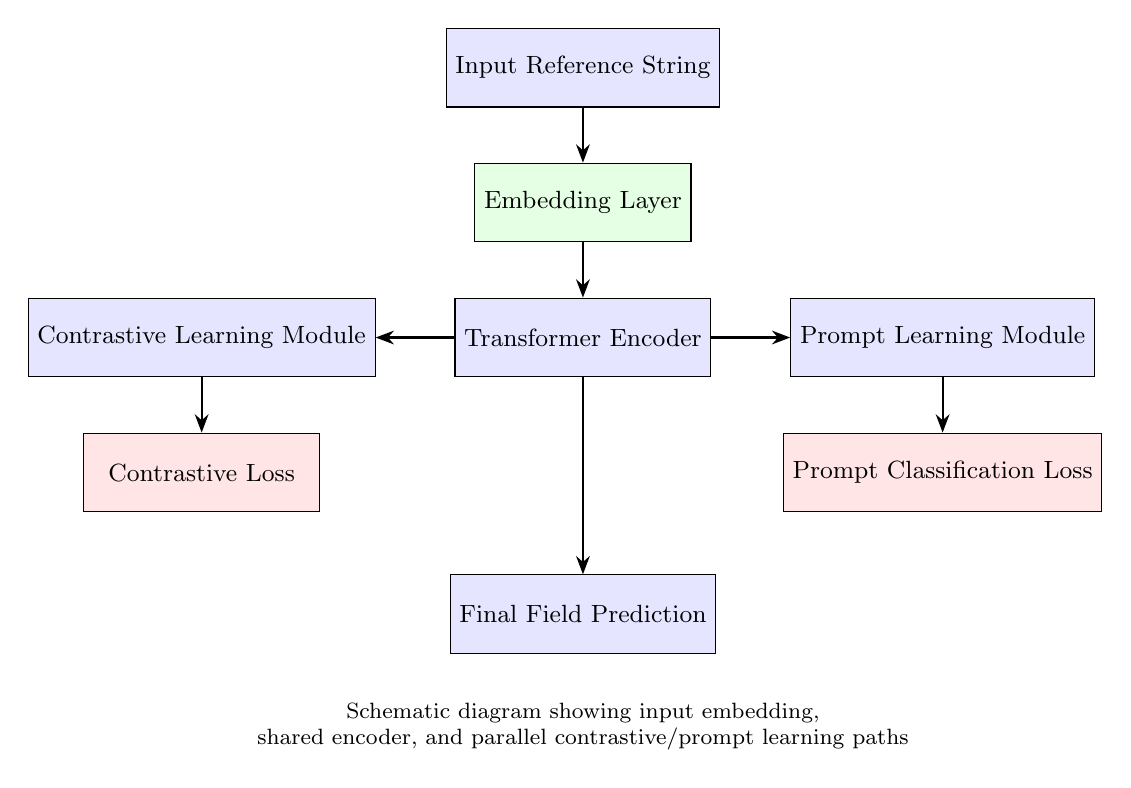
\begin{tikzpicture}[node distance=0.7cm and 1.4cm, every node/.style={font=\small},
    process/.style={rectangle, draw, minimum height=1cm, minimum width=2.5cm, fill=blue!10, text centered},
    embedding/.style={rectangle, draw, minimum height=1cm, minimum width=2.5cm, fill=green!10, text centered},
    loss/.style={rectangle, draw, minimum height=1cm, minimum width=3cm, fill=red!10, text centered},
    arrow/.style={->, thick, >=Stealth}]

% Input section
\node[process] (input) {Input Reference String};
\node[embedding, below=of input] (embed) {Embedding Layer};
\node[process, below=of embed] (encoder) {Transformer Encoder};

% Split branches
\node[process, right=1cm of encoder] (prompt) {Prompt Learning Module};
\node[process, left=1cm of encoder] (contrast) {Contrastive Learning Module};

% Output heads
\node[loss, below=of prompt] (promptloss) {Prompt Classification Loss};
\node[loss, below=of contrast] (contrastloss) {Contrastive Loss};

% Final prediction
\node[process, below=2.5cm of encoder] (prediction) {Final Field Prediction};

% Arrows
\draw[arrow] (input) -- (embed);
\draw[arrow] (embed) -- (encoder);
\draw[arrow] (encoder) -- (prompt);
\draw[arrow] (encoder) -- (contrast);
\draw[arrow] (prompt) -- (promptloss);
\draw[arrow] (contrast) -- (contrastloss);
\draw[arrow] (encoder) -- (prediction);

% Legends (optional)
\node[align=center, font=\footnotesize, below=0.5cm of prediction] {Schematic diagram showing input embedding,\\ shared encoder, and parallel contrastive/prompt learning paths};

\end{tikzpicture}
    \caption[\texttt{CONT\_Prompt\_ParsRef}: contrastive and prompt learning architecture]{Overview of the CONT\_Prompt\_ParsRef architecture combining contrastive and prompt learning.}
    \label{fig:contrastive-learning}
\end{figure}
% While BiLSTM and Transformer-based models have been responsible for most of the recent progress in bibliographic reference parsing, Yin and Wang~\cite{contrastive} presented a novel approach that includes contrastive learning and prompt-based learning for segmentation.
% \texttt{CONT\_Prompt\_ParsRef} is their model that aims to enhance the robustness of the model, especially in low-resource settings and multilingual citation styles, by making representations more discriminative and more interpretable. The contrastive learning component clusters similar entity tokens in the embedding space and separates dissimilar ones, which helps the model to find the difference between ambiguous or overlapping field types. Meanwhile, the prompt learning mechanism helps the model use templated prompts embedded within the input, which allows it to learn from few-shot examples or external guidance.
% The authors validated their methods on a bilingual benchmark dataset containing 12,000 reference strings each for Chinese and English. Compared to BiLSTM + CRF and BERT + CRF baselines, their model achieved more than 96\% F1 scores for both sets of languages. Their study confirmed that both modules (contrastive and prompt learning) made considerable contributions towards the performance of the model. Moreover, their system has good generalization to different citation styles. This work is a breakthrough in the sense that it demonstrates that more recent representation learning techniques from larger NLP research can be easily applied to bibliographic parsing tasks.

\section[Comparative Evaluations and Modern Architectures]{Comparative Evaluations\\ and Modern Architectures}
Following up on Neural ParsCit’s~\cite{prasad2018neuralparscit} observations, recent work has focused on the task of comparatively assessing modern NLP architectures for reference parsing. In particular, Cuéllar Hidalgo et al. (2024)~\cite{ArchComapre} conducted an empirical comparison of three well-known architectures: CRF, BiLSTM + CRF, and Transformer + CRF. Their study used the gigantic GIANT corpus~\cite{giant} (comprising over 900 million annotated references across 1500+ citation styles) for training and the well-established CORA corpus~\cite{cora1999} for testing.
Their findings once more validated the superiority of BiLSTM + CRF over pure CRF models in identifying complex syntactic structures in reference strings. What was more interesting, Transformers-based models showed competitive performance but did poorly in cases with limited labeled data or noisy labels, which indicated that even with their theoretical advantages, Transformers still need a lot of careful tuning or more training data to outperform BiLSTMs in this use case.
Perhaps one of their most significant contribution was to standardize preprocessing and consistent testing for all models. This way, it helped us to know that performance differences were because of the architectural differences between the models and not the inconsistencies in the data. These experiments also pointed out the importance of embedding techniques, using Byte-Pair Encoding with character-level features, which enhanced the performance of all models in handling token-level irregularities, such as hyphenated names or Roman numeral volume numbers.

\section{Other Tools and Alternative Approaches}
In addition to traditional and neural sequence models, several other systems have explored new directions. The ParsRec approach~\cite{ParsRec} suggested a meta-learning system that proposes the best parser (out of a set of candidate systems) for a specific reference string, according to metadata and structural information. This is part of a growing tendency towards ensemble and hybrid solutions that take advantage of the strengths of different tools.
In addition, software like GROBID~\cite{grobid} and AnyStyle~\cite{anystyle} have become very popular due to their simplicity and deployment in digital library pipelines. AnyStyle is especially valuable because it employs a hybrid approach with the utilization of hand-crafted features that serve as input into a CRF model, and simple training on proprietary datasets. Its adaptability and low-resource suitability make it suitable for libraries that have specialized citation formats or non-English content.

\section{Summary and Open Challenges}
In short, the field of bibliographic reference string parsing has progressed from rule-based and HMM to CRFs and, more recently, to neural models such as BiLSTM and transformer models. Each has addressed problems of the previous generation, from lack of generalization to dependence on hand-engineered features.
But there remain issues, most systems get trained and tested on English-language datasets mostly, and noisy or OCR-extracted references are still a concern. While neural models generalize more, they are data hungry and may not work well in low-resource environments. Finally, deployment in real workflows (citation indexing, digital repositories) required robust tools that compromise between accuracy, speed, and flexibility.
In our work, we attempt to further explore this balance by re-examining the value of hand-engineered features, like in models such as AnyStyle, and putting their cooperation with modern neural frameworks to the test. We hope that by integrating structured, interpretable features into data-driven learning, we can build models that are both efficient and practical in a wide range of bibliographic scenarios.

\cleardoublepage

\chapter{Methodology}
\label{ch:methodology}

\section{System Architecture}
The goal of this system is to convert unstructured reference strings into structured bibliographic metadata by the process of assigning each token with its corresponding semantic field (e.g., author, title, publisher, year). This task is framed as a sequence labeling problem, and the model learns to create field-level labels for a string of tokens to produce labeled output that can be consumed by digital libraries, citation indexes, or metadata extraction programs.
The system architecture is composed of modular stages: input ingestion and preprocessing, hand-engineered feature extraction, contextual embedding generation, feature concatenation, and token-level sequence modeling with supervised learning models. The stages are designed to be extendable and flexible in order to facilitate exploration with various types of embeddings, feature sets, and model architectures.

\subsection{Input and Dataset Constraints}
The system uses the GIANT dataset~\cite{giant}, which is one of the largest annotated reference string corpora available in this field anywhere. The complete GIANT corpus is made up of more than 900 million citations covering thousands of scientific styles and topics. However, due to computational constraints, it was not possible to train models on the entire corpus. A random sample of 5 million citation strings was chosen to ensure high diversity among citation styles, fields, and languages. Effective experimentation was conducted at this scale while preserving the dataset’s challenging variability.
All the strings in the dataset are first annotated in an XML-based hierarchical format that provides field-level segmentation, but it’s not directly compatible with the standard sequence labeling formats. The XML annotation has both the main labels mentioned previously and additional metadata or formatting tags that are not relevant to the core parsing task. As a processing step, the extra labels were removed, and the remaining of the string turned into a flat reference.

Annotated reference string before parsing example: 
\begin{verbatim}
    <author>
        <family>Ritchie</family>,
        <given>E.</given> and
        <family>Powell</family>,
        <given>Elmer Ellsworth</given>
    </author> (
    <issued>
        <year>1907</year>
    </issued>)
    <title>Spinoza and Religion.</title>
    <container-title>The Philosophical Review</container-title>,
    <volume>16</volume>(
    <issue>3</issue>), p.
    <page>339</page>. [online] Available from:
    <URL>http://dx.doi.org/10.2307/2177340</URL>
\end{verbatim}
Annotated reference string after parsing example:
\begin{verbatim}
    <author>
        Ritchie E. and Powell, Elmer Ellsworth
    </author>
    <punc>
        (
    </punc>
    <year>
        1907
    </year>
    <punc>
        )
    </punc>
    <title>
        Spinoza and Religion.
    </title>
    <container-title>
        The Philosophical Review
    </container-title>
    <volume>
        16
    </volume>
    <punc>
        (
    </punc>
    <issue>
        3
    </issue>
    <punc>
        )
    </punc>
    <punc>
    ,
    </punc> 
    <page>
        p. 339
    </page>
    <other>
        [online] Available from:
    </other>
    <URL>
        http://dx.doi.org/10.2307/2177340
    </URL>
\end{verbatim}
And then turned into a token-level BIO tagging scheme. In this scheme, every token is labeled as the beginning (B-) or inside (I-) of some field, or as outside (O) if it does not belong to an identified segment. This conversion was performed in order to get the data into a format that can be used with off-the-shelf sequence labeling models. Some of the last tags are B-Author, I-Title, B-Journal, and B-Year. By using BIO encoding, the models are able to learn fixed field boundaries in citation strings, even across highly varying formatting styles.

\subsection{Preprocessing and Tokenization}
Raw reference strings can be different in the way they’re formatted, their punctuation, and the language, which makes preprocessing an important step. The tokenization method used in the system is whitespace-sensitive, punctuation-sensitive, and character pattern-sensitive. This makes sure that tokens like initials, abbreviations, hyphenated names, volume/issue numbers, and DOIs are appropriately separated and paired with the correct label.
All the special characters and punctuation are kept unless otherwise filtered because they can have essential roles in delimiting fields. For instance, the presence of parentheses for a year, or quotation marks for a title, often serves as an implicit indicator that is useful to handcrafted features as well as learned representations.

\subsection{Feature Extraction}
One of the innovations of this system lies in its use of hand-engineered features inspired by the AnyStyle~\cite{anystyle} reference parsing framework. AnyStyle has been proven to perform well with lightweight CRF models that are guided by feature sets that are carefully crafted by hand. In this project, the same strategy is followed, and features that are domain-aware and structurally informative are derived.
The feature space includes:
\begin{description}
\item[Orthographic features:] capitalization, digits, punctuation types.
\item[Lexical cues:] dictionary matches on publication names, author names, or publication types that are common.
\item[Positional features:] token position from the start/end of the string, section, position.
\item[Contextual features:] features from the preceding and following tokens.
\end{description}
These are generated for each token within the reference string and encoded into a sparse vector format. They are primarily used for adding domain-specific patterns into the learning process, especially useful for rare citation styles and unusual formatting.

\subsection{Embedding Generation and Feature Fusion}
In addition to hand-engineered features, the system uses contextual embeddings to acquire deeper semantic and syntactic relationships. Two embedding methods are explored:
\begin{enumerate}
\item Byte-Pair Encoding (BPE)~\cite{bpemb} embeddings: Subword embeddings that are robust to out-of-vocabulary, low-frequency, or unknown words. BPE is found to be beneficial in bibliography information, where there are many domain- or author-related words with low frequencies.
\item BERT~\cite{2019-bert} embeddings: Pre-trained contextual embeddings based on the Transformer architecture. BERT captures long-range dependencies and subtle meaning from the entire sentence context. Its success in numerous NLP applications encourages its application in this reference parsing pipeline.
\end{enumerate}
These embeddings can be used individually or combined with the hand-engineered features to produce a joint token representation. This combination enables the system to take advantage of both data-driven learning and domain-guided structure, making use of both approaches.

\subsection{Sequence Labeling and Output}
The final step of the system is sequence labeling, in which the token representations are input into one of the supervised models:
\begin{itemize}
\item Conditional Random Fields (CRF)~\cite{crf2001}: A strong baseline for structured prediction, especially with hand-engineered features.
\item BiLSTM + CRF: A deep learning model that captures bidirectional context and combines it with a structured output layer.
\end{itemize}
These models are trained using annotated reference strings to learn the transition patterns between labels and to predict the correct field label for each token. The output is a sequence in which each token is marked up with its label.

\begin{figure}[ht]
    \centering
    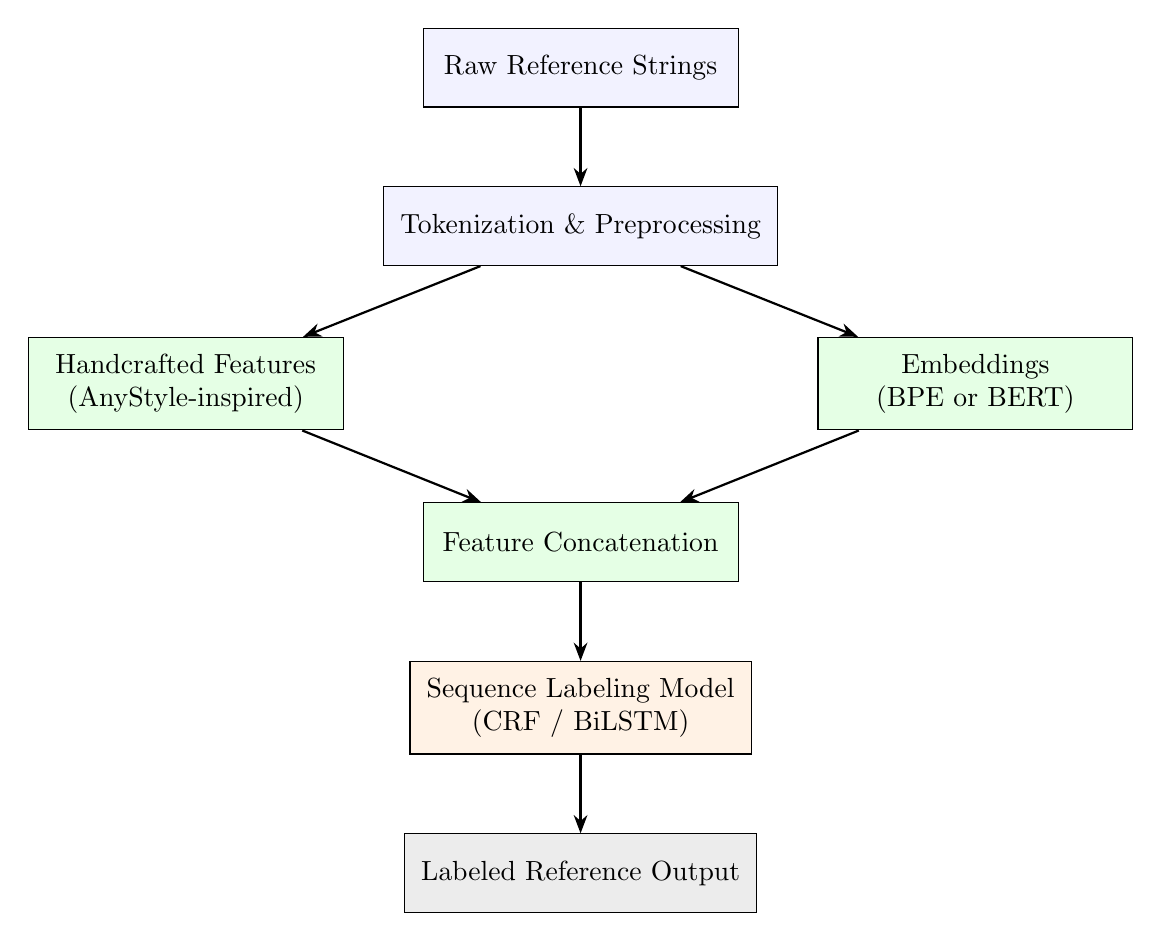
\begin{tikzpicture}[node distance=1.5cm]

\tikzstyle{inputnode} = [rectangle, draw, fill=blue!5, text centered, minimum width=4cm, minimum height=1cm, align=center, inner sep=6pt]
\tikzstyle{featurenode} = [rectangle, draw, fill=green!10, text centered, minimum width=4cm, minimum height=1cm, align=center, inner sep=6pt]
\tikzstyle{modelnode} = [rectangle, draw, fill=orange!10, text centered, minimum width=4cm, minimum height=1cm, align=center, inner sep=6pt]
\tikzstyle{outputnode} = [rectangle, draw, fill=gray!15, text centered, minimum width=4cm, minimum height=1cm, align=center, inner sep=6pt]

% Nodes
\node (input) [inputnode] {Raw Reference Strings};
\node (token) [inputnode, below=1cm of input] {Tokenization \& Preprocessing};
\node (features) [featurenode, left=0.5cm of token, yshift=-2cm] {Handcrafted Features\\ (AnyStyle-inspired)};
\node (embedding) [featurenode, right=0.5cm of token, yshift=-2cm] {Embeddings\\ (BPE or BERT)};
\node (fusion) [featurenode, below=3cm of token] {Feature Concatenation};
\node (model) [modelnode, below=1cm of fusion] {Sequence Labeling Model\\ (CRF / BiLSTM)};
\node (output) [outputnode, below=1cm of model] {Labeled Reference Output};

% Arrows
\draw [arrow] (input) -- (token);
\draw [arrow] (token) -- (features);
\draw [arrow] (token) -- (embedding);
\draw [arrow] (features) -- (fusion);
\draw [arrow] (embedding) -- (fusion);
\draw [arrow] (fusion) -- (model);
\draw [arrow] (model) -- (output);

\end{tikzpicture}

    \caption{System architecture for reference string parsing.}
    \label{fig:system-architecture}
\end{figure}
\cleardoublepage

\section{Feature Engineering}

Feature engineering is vital to the reference parsing system introduced in this work. The bibliographic reference segmentation is a prediction problem, one where the model must assign a field-level label (author, title, year, etc.) to each token in a sequence. In order to be able to do this efficiently, the model requires informative representations of each token, those representations should capture both the token’s content and its contextual significance.

In the past few years, there has been a growing popularity in employing deep contextual embeddings like BERT~\cite{2019-bert} to embed text in natural language processing tasks. Even in tasks like citation parsing, where structure and formatting have strong semantic clues, traditional hand-engineered features can still have a significant value. They extract surface information that is often consistent across citation styles, like punctuation patterns, capitalization, or token order.

To gain a balance between generalization and interpretability, our system uses two types of features:
\begin{enumerate}
\item A set of \textbf{handcrafted features} inspired by the AnyStyle~\cite{anystyle} citation parser.
\item \textbf{Learned embeddings} derived from either subword-level models (BPE)~\cite{bpemb} or deep contextual models (BERT)~\cite{2019-bert}.
\end{enumerate}
In the following sections, we describe each feature group in detail, beginning with the handcrafted features.

\subsection{Handcrafted Features}
In this work, one of the design decisions was to complement neural embeddings with a robust set of hand-engineered features. These features provide interpretable, low-level cues that are very useful for detecting structural patterns in citation strings, patterns that are often overlooked ot inconsistently represented in pretrained language models. Our approach to feature engineering is influenced by AnyStyle, an open-source library for citation parsing developed by Sylvester Keil~\cite{anystyle}.

AnyStyle models citation parsing as a sequence labeling task and relies on a CRF model that has been trained on a wide range of citation styles. Unlike neural architectures, which can rely a lot on pretraining and embeddings, AnyStyle achieves high performance through a well-crafted set of features that encode orthographic, lexical, and contextual information.
These include features such as token capitalization, punctuation patterns, and dictionary lookups, all these features are designed to enable the model to detect bibliography entities in different types of citations.

In our system, we take and extend this method by constructing a set of features to feed into the model, concatenated with subword and contextual embeddings. This mixed representation allows the model to take advantage of deep contextual understanding through embeddings and interpretable surface signals from the hand-engineered features.
To facilitate compatibility, we re-implemented a subset of AnyStyle’s feature classes, modifying or adding to some where necessary.

In the following sections, we’ll describe each feature class, its role, and how it helps in the overall reference parsing task. 

\subsubsection{Affix Feature}
The affix feature extracts fixed-length prefixes and suffixes of tokens. It is useful for recording common patterns in names, abbreviations, or technical terms that appear repeatedly in bibliography citations. For instance, author initials like “J.” or “Ph.”, or journal abbreviations like “IEEE” or “JMLR”, have a specific pattern at the start or end of words.
This feature works by taking a number of characters from the beginning (prefix) or end (suffix) of the token. In our case, two variations of this feature class were applied: one that takes the first two characters (prefix) from the token, and another one that takes the last two characters (suffix) from the token. These affix pieces are built up incrementally–so the prefix extractor for a token like “Journal” would extract “J” and “Jo”, and the suffix extractor would extract “l” and “al”.

Affix features make the model able to generalize to out-of-vocabulary tokens by picking up on subword patterns that could indicate specific field types. For example, journal names often have a shared suffix like “-ology” or “-ics”, and author names often have a predictable pattern of abbreviations. While it’s simple in structure, these features are helpful in field prediction, especially where token-level embeddings on their own can sometimes lack attention to detail.

\subsubsection{Brackets Feature}
The brackets feature captures data on whether a token is enclosed by or adjacent to typical bracket symbols, such as parentheses \texttt{()}, square brackets \texttt{[]}, or angle brackets \texttt{<>}. This is a useful feature because citation formats could put some metadata in brackets – e.g., publication years, volume numbers, or reference indices – to visually distinguish them from other fields.
This feature adds a tag to the token, such as \texttt{parens}, \texttt{square-brackets}, \texttt{angle}, or more specific tags such as \texttt{opening-paren}, \texttt{closing-square-bracket}, etc., depending on the shape of the token. For example, the token (2003) would be tagged as \texttt{parens}, and a token starting with \texttt{[} would be tagged as \texttt{opening-square-bracket}.
Tokens without any brackets are simply tagged as \texttt{none}. When the token does not belong to one of the typical patterns, it is tagged as \texttt{other}.

By flagging bracket types and positions, this feature enables the model to recognize common citation patterns, like parenthesized years or square-bracketed reference numbers, that are used across many citation styles. This kind of formatting hint is sometimes necessary to help get an accurate segmentation and recognize which field this token might belong to, especially in noisy or reference strings extracted using OCR.

\subsubsection{Canonical Feature}
The canonical feature provides a normalized representation of each token by removing accents and converting it to a standardized, lowercase form. The main goal is that tokens of the same structure or meaning are treated in the same way by the model, whether they appear different due to language, style, or formatting differences.
In order to achieve this, the feature captures the first shape of the token (before any change) and performs some normalization operations. It initially performs Unicode normalization to break the characters down to their base form – i.e., separating a letter from its accent marks. It then removes all the accents and other diacritical marks, retaining only the base characters.
Finally, it scrubs the string of any additional formatting noise and makes it lowercase.

For instance, the name \texttt{García} is shortened into \texttt{garcia}, and \texttt{MÜLLER} to \texttt{muller}. This makes it easier for the model to recognize that these are likely the same name or entity with minor stylistic or typographic differences.
This capability proves useful, especially while tokenizing citations with names, titles, or journal names in multiple languages or styles. It minimizes inconsistency in the input and allows the model to generalize more effectively over the large variety of tokens found in citation strings.

\subsubsection{Caps Feature}
The caps feature tracks information about the capitalization pattern of each token. Capitalization tends to be an effective cue in reference strings — i.e., it can signal the occurrence of names, acronyms, or stylized title spacing. By observing and categorizing these patterns, the model has the ability to enhance on identify between different types of fields such as author names, journal names, or abbreviations.

This property works by looking at the original shape of the token and assigning one of a set of classes depending on whether and where there is one or more uppercase letters:
\begin{compactitem}
\item \textbf{single:} A single uppercase letter (e.g., \texttt{J}), common in shortened names or initials.
\item \textbf{initial:} A token that starts with an uppercase letter followed by a lowercase letter (e.g., \texttt{John}), typically used for names or title-cased words.
\item \textbf{caps:} A word token that consists entirely of all capital letters (e.g., \texttt{IEEE}, \texttt{SCIENCE}), typically delimiting acronyms or publication titles.
\item \textbf{lower:} A word token consisting only of lowercase letters (e.g., \texttt{and}, \texttt{volume}), typically less informative in a stand-alone.
\item \textbf{other:} An extra bucket for anything token-wise not accommodated by the above patterns, e.g., words of mixed cases, numbers, or punctuation.
\end{compactitem}

By assigning tokens to these capitalization classes, the model is more likely to correctly infer the possible function of a token within a citation, particularly when combined with other structural or contextual information.

\subsubsection{Category Feature}
The category feature determines Unicode character type of the first and last token characters to yield basic structural details. Through this analysis, the model achieves token classification based on characters, which provides information about first-letter identification and terminal punctuation, and symbol and number presence.

The feature retrieves the first and last tokens and then assigns them to the appropriate Unicode general categories through its mapping process. The Unicode general categories cover uppercase letters (\texttt{Lu}), lowercase letters (\texttt{Ll}), modifier letters (\texttt{Lm}), numbers (\texttt{N}), punctuation types (\texttt{P}, \texttt{Pc}, \texttt{Pd}, etc.), symbols (\texttt{S}), and unspecified other categories. Character data that cannot be categorized goes under the category of \texttt{none}.

For example:
\begin{compactitem}
\item When applied to \texttt{Vol.} the Vol. feature would provide output as \texttt{Lu} for \texttt{V} and \texttt{P} for the period.
\item The token 2023) provides both \texttt{N} as a number category and \texttt{Pe} for parenthesis.
\end{compactitem}
The model can apply its knowledge to numerous token forms because this feature ignores token content. The reference string benefits from this feature if it contains structured formatting cues that indicate field boundaries or field types through specific brackets or numbers and characters.

\subsubsection{Dictionary Feature}
The dictionary feature tries to see if a token matches a known word in a collection of lists that includes names, places, publishers, and journal names. The lists are being read from a dictionary file, grouped into the lists mentioned above. It is useful for detecting entities that would show up in a frequent way in reference strings, such as publisher names, city names of publication, or common journal abbreviations.
Each token is compared and checked to see if it exists in one of these lists:
\begin{compactitem}
\item \textbf{name} - common first or last names in the author field
\item \textbf{place} - cities or locations typically in publisher field
\item \textbf{publisher} - publishing firm or organisation names
\item \textbf{journal} - full journal titles or journal abbreviations
\end{compactitem}
If a token exists in one of the lists, it is marked as \texttt{T} (true) for that category; otherwise, it’ll be marked \texttt{F} (false). The output vector from this feature will have four components, each referencing one of the dictionary categories.
For example, token \texttt{Springer} might return \texttt{[F, F, T, F]}, which indicates that there is a match in the publisher dictionary but not in other dictionaries. This feature will allow the model to create a connection between a token with a role for it, which could lead to an increase in accuracy in the field segmentation.

The dictionary lists are extracted from structured reference data and preprocessed for consistency. Although these features are not very reliable and couldn’t be sufficient to provide correct labeling, they help with adding precision signals when used with contextual or structural features.

\subsubsection{Keyword Feature}
The keyword feature uses keyword patterns to assess token classification regarding previously known semantic categories. This detection method is intended to identify particular metadata signals within citation strings by analyzing both words and symbols.

The internal operation uses pre-determined groups of regular expressions that control category matching. The semantic roles (\texttt{editor}, \texttt{journal}, \texttt{date}, \texttt{volume}) exist as separate categories, and the system checks each token against different language versions of relevant keywords. Editor-related terminology in the metadata section contains multiple English designs, including \texttt{ed.}, \texttt{editors}, and \texttt{edited}, in addition to German (\texttt{herausgeber}) and Spanish or French equivalents (\texttt{compilador}). The grammar accepts character sequences from the symbolic series and the CJK series.
This feature evaluates by testing every pattern one by one until it encounters a category expression that perfectly matches the current token. The feature operates without producing an output whenever no suitable matching pattern exists.
Some example categories include:
\begin{compactitem}
\item \textbf{editor:} tokens like \texttt{ed.}, \texttt{Hrsg.}
\item \textbf{volume:} \texttt{vol.}, \texttt{no.}, \texttt{issue}, \texttt{heft}
\item \textbf{date:} matches several months or season names such as \texttt{May}, \texttt{Fall}, and \texttt{Herbst}.
\item \textbf{journal:} words like \texttt{Journal}, \texttt{Quarterly}, \texttt{Review}, or \texttt{Zeitschrift}
\item \textbf{accessed:} metadata like \texttt{retrieved}, \texttt{accessed}, \texttt{abgerufen}.
\item \textbf{locator:} \texttt{doi}, \texttt{url}
\item \textbf{etal:} short forms like \texttt{et al.}, \texttt{others}
\end{compactitem}
Through this feature, the model gains enhanced semantic cues, which improve its ability to detect tokens with functional significance above visual presentation form. The feature precisely detects citation components, especially for their publication placement (\texttt{in}) as well as their authorship (\texttt{author}, \texttt{editor}, \texttt{translator}) and reference access methods (\texttt{url}, \texttt{arxiv}, \texttt{pubmed}).
Tokens that match the established keyword categories function as strong indicators for the field, but only some tokens have matching entries.

\subsubsection{Locator Feature}
The Locator function identifies persistent digital identifiers along with external resource pointers that function as tokens. The system contains the main groups of locators: DOIs, URLs, ISBNs, and PubMed IDs, along with additional academic citation locator types. Recognition of these tokens is vital because they most commonly occur at citation endings while holding semantic and structural differences from the rest of the fields.
The feature uses regular expression patterns to detect persistent digital identifiers, which also include commonly used external resource pointers:
\begin{compactitem}
\item The token detection system verifies terms which include \texttt{DOI}, \texttt{ISBN}, \texttt{URL}, \texttt{PMCID} and \texttt{PubMed}.
\item A Digital Object Identifier stands as \texttt{10.} followed by a numeric prefix and a suffix which combines as \texttt{10.1000/xyz123}.
\item The feature detects typical URI forms which start with \texttt{http://}, \texttt{https://}, or \texttt{ftp://} within web addresses.
\end{compactitem}
The feature returns \texttt{'T'} (true) when any defined patterns match within the analyzed token, indicating a potential locator. Otherwise, it returns \texttt{'F'} (false).
Example:
\begin{compactitem}
\item \texttt{https://doi.org/10.1007/s00799-018-0242-1} → \texttt{T}
\item \texttt{PMID: 12345678} → \texttt{T}
\item \texttt{Springer} → \texttt{F}
\end{compactitem}
Through this feature, the model detects tokens containing external source references and accesses information, thus enhancing its ability to accurately classify fields, particularly for digital and web-based references.

\subsubsection{Number Feature}
The number feature categorizes tokens based on whether and how there is numerical information. Numbers are essential in the middle of many bibliographic fields — e.g., years, volume numbers, ranges of pages, ISBNs, or identifiers — and understanding their format can help the model to decide the token's likely function in a citation. This feature applies a series of pattern-matching rules to translate all numeric tokens into a particular category. Some of the main categories include:
\begin{compactitem}
\item \textbf{volume:} Tokens that have the appearance of a volume and issue format, such as \texttt{12(3)} or \texttt{5:7}.
\item \textbf{isbn:} Strings that conform to the pattern of ISBN numbers, both starting with \texttt{978} and those starting with \texttt{979}.
\item \textbf{year:} Four-digit years from a reasonable range of history, such as \texttt{1998} or \texttt{2023}.
\item \textbf{quad, triple, double, single:} Tokens made up of 4, 3, 2, or 1 digits respectively. These simple forms typically represent years, page numbers, or brief identifiers.
\item \textbf{all:} Tokens made entirely of digits, but not in one of the other specialized forms.
\item \textbf{range:} Numerical ranges with hyphens, e.g., \texttt{123–145}, commonly page numbers.
\item \textbf{idnum:} Alphanumeric identifiers in which a number is prefixed with letters or codes, e.g., \texttt{ABC-123} or \texttt{ISSN2049}.
\item \textbf{ordinal:} Numerical and alphabetical combination tokens, e.g., \texttt{3rd}, \texttt{21st}, or \texttt{2a}, appearing infrequently in editions or titles.
\item \textbf{numeric:} Tokens having at least one digit but none of the preceding patterns.
\item \textbf{roman:} Roman numerals like \texttt{III}, \texttt{XIV}, or \texttt{iv}, appearing infrequently to number chapters, volumes, or appendices.
\end{compactitem}
Otherwise, if the token does not belong to any known numeric pattern, it gets labeled as \texttt{none}.

By classifying these fine-grained numeric types, the model gains a deeper sense of the organization of the reference, having the ability to distinguish between a publication year, an ISBN, and a volume/issue number, even when all appear to be numbers. This helps to improve the precision of field classification, especially for citation styles that vary in the way and where numbers appear.

\subsubsection{Position Feature}
The position feature holds the relative location of a token within the reference string. In citation parsing, when a token's position can powerfully predict its role, its position tends to reveal a great deal about its function. Authors' names tend to be toward the front, say, whereas publication dates, URLs, or page numbers tend to appear closer to the end.
This feature gives back one of the following values, depending on the token's position in the sequence:
\begin{compactitem}
\item \textbf{only:} If the token is the only token in the sequence
\item \textbf{first:} If the token is the first token in the sequence
\item \textbf{last:} If the token is the last token in the sequence
\item \textbf{A relative position value} (as an integer between 0 and 10) if the token is in the middle somewhere
\end{compactitem}
The relative position is calculated as a coarse-grained proportion: the index of the token divided by the number of tokens and adjusted by an absolute level of precision (for example, 0 to 10). As an example, a token in the middle of a sequence of 20 tokens would receive the value 5.

By exposing the model to this positional information, the feature helps the model learn to recognize in which portions of a reference string one will most likely discover specific types of information. This can be extremely helpful in free-form or otherwise variably styled references, where even the formatting cannot give sufficient indication for field separation.

\subsubsection{Punctuation Feature}
The punctuation feature recognizes the presence and type of punctuation in a token. Punctuation will generally play a structural role in citation strings, separating fields or designating formatting conventions. For example, colons will separate titles and subtitles, periods will designate abbreviations, and hyphens will denote ranges like page numbers or dates.
The feature looks at each token and labels it based on the punctuation that it contains:
\begin{compactitem}
\item \textbf{none:} The token does not have any punctuation.
\item \textbf{colon:} The token contains a colon (\texttt{:}), which is used for title or subtitle delineation.
\item \textbf{hyphen:} The token contains a hyphen or dash, which can indicate a range (i.e., \texttt{123–145}) or be part of a compound word.
\item \textbf{period:} The token contains a period (\texttt{.}), which can indicate abbreviations or sentence finality.
\item \textbf{amp:} The token has an ampersand (\texttt{\&}), often used to join author names (e.g., \texttt{Smith \& Johnson}).
\item \textbf{other:} The token has punctuation not in one of the above classes.
\end{compactitem}
By capturing these distinctions, the punctuation feature provides useful cues to token boundaries, field separators, and potential abbreviations — all of which are useful to the model in annotating different parts of a citation.

\subsubsection{Terminal Feature}
Terminal property identifies in which way a token is terminating, namely if it is terminating in punctuation, brackets, or quotes. In citations of bibliography, the punctuation a token is terminating in often signals the end of a field or the separation between units of meaning, e.g., the end of an author name, title, or publication date.
This feature looks at the trailing characters of the token and categorizes it as one of four based on the quality of the ending punctuation it possesses:
\begin{compactitem}
\item \textbf{strong:} The token contains a strong punctuation mark such as a period (\texttt{.}), closing parenthesis (\texttt{)}), or square bracket (\texttt{]}), possibly followed by a quotation mark. These tend to mark the end of a field or sentence.
\item \textbf{moderate:} The token is suffixed with a quotation or colon. It may be preceded by a lighter punctuation character at times. These may mark a transition, like the start of a subtitle or inline citation.
\item \textbf{weak:} The token is preceded by a lighter punctuation character like a comma, semicolon, hyphen, or exclamation mark. These mark continuation but can still segment parts of a field.
\item \textbf{none:} The token ends without any meaningful punctuation.
\end{compactitem}
For example:
\begin{compactitem}
\item \texttt{2023).} → \texttt{strong}
\item \texttt{"Chapter 2:} → \texttt{moderate}
\item \texttt{Vol. 5,} → \texttt{weak}
\item \texttt{Science} → \texttt{none}
\end{compactitem}
By maintaining these distinctions, the terminal feature helps the model to learn where fields most likely begin or end, especially in citation styles where such patterns are not absolutely dictated by format but instead are a function of punctuation. It plays a silent but important role in improving the accuracy of token labelling across citation formats.
\clearpage

\subsection*{Summary of Handcrafted Features}
The new hand-crafted features employed in this work are inspired by how reference parsing is addressed in AnyStyle~\cite{anystyle}, but are reworked and extended to more effectively meet the needs of modern neural models. They encode a dense array of linguistic, structural, and semantic cues — including orthographic features, token position, punctuation, character types, and semantic dictionaries. Each of these provides a different perspective on the reference string, and together they form a dense representation that allows accurate field labeling independent of citation style. Later, we evaluate the contribution of these features in isolation as well as in combination with embedding-based methods.
\renewcommand{\arraystretch}{1.3}
\begin{table}[ht]
\centering
\caption[Summary of Handcrafted Features]{Summary of handcrafted features used in the citation parsing model}
\label{tab:handcrafted-features}
\begin{tabular}{p{4cm}p{10cm}}
\toprule
\textbf{Feature} & \textbf{Description} \\
\midrule
\texttt{AffixFeature} & Extracts prefixes and suffixes from each token to detect morphological patterns and common abbreviations. \\
\texttt{BracketsFeature} & Identifies tokens enclosed in or adjacent to brackets like \texttt{()}, \texttt{[]}, or \texttt{<>}, often used for years or references. \\
\texttt{CanonicalFeature} & Produces a normalized lowercase version of the token without accents or formatting noise. \\
\texttt{CapsFeature} & Classifies tokens based on capitalization, e.g., all-caps, initials, or lowercase. \\
\texttt{CategoryFeature} & Returns the Unicode category of the first and last character, helping to detect punctuation, digits, or letters. \\
\texttt{DictionaryFeature} & Checks if a token exists in domain-specific dictionaries: names, publishers, journals, or places. \\
\texttt{KeywordFeature} & Matches tokens against keyword patterns to detect roles like editor, translator, journal, or date terms. \\
\texttt{LocatorFeature} & Detects persistent identifiers like DOIs, URLs, PubMed IDs, and ISBNs. \\
\texttt{NumberFeature} & Classifies numeric tokens (e.g., years, volumes, page ranges, Roman numerals) based on their structure. \\
\texttt{PositionFeature} & Encodes the position of a token within the reference string (first, last, middle, etc.). \\
\texttt{PunctuationFeature} & Identifies punctuation within a token (colon, hyphen, ampersand, etc.). \\
\texttt{TerminalFeature} & Examines how a token ends to infer punctuation strength and field boundaries. \\
\bottomrule
\end{tabular}
\end{table}
\renewcommand{\arraystretch}{1.0}



\clearpage

\subsection{Embedding-Based Features}
Embedding-based features provide dense, learned token representations through embedding semantic and contextual details. Contrary to handcrafted features that rely on surface patterns and professional knowledge, embeddings are learned in large bodies of text and may involve subtle language use, structural dependencies, and sense. In this paper, we experiment with two types of embeddings: Byte-Pair Encoding (BPE) embeddings and BERT-based contextual embeddings. These embeddings are used alone or blended with hand-crafted features to enhance the model's ability to label tokens appropriately in reference strings.

\subsubsection{Byte-Pair Encoding (BPE) Embeddings}
Byte-Pair Encoding (BPE) embeddings offer a tokenization-free, light, and multilingual way of subword representation. We incorporate in this paper pre-trained BPE embeddings released by the BPEmb project, which offers subword-level vector representations for 275 languages, including low-resource languages~\cite{bpemb}.
BPE is a data-driven compression algorithm that continuously merges the most frequent adjacent symbol pairs in a sequence. For example, in English, the most frequent pair, such as \texttt{t} and \texttt{h} might be merged into \texttt{th}, then further pairs such as \texttt{th} and \texttt{e} into \texttt{the}, depending on frequency. The number of merge operations the unit receives will determine its granularity as a subword unit, with fewer being more finely grained at the character level and more being units that are more like whole words~\cite{bpemb}.

BPEmb takes advantage of this idea to split untokenized, raw Wikipedia text into many languages and then learns embeddings across subword units using the GloVe algorithm~\cite{bpemb,glove}. The method has the following significant advantages:
\begin{compactitem}
\item \textbf{No whole-word tokenization required,} especially suitable for languages without word boundaries (for example, Chinese, Japanese).
\item \textbf{Multilinguality,} with embeddings trained over a wide variety of languages, ranging from high-, medium-, and low-resource languages.
\item \textbf{Compact size,} outperforming other models like FastText in certain languages while using significantly less memory (e.g., 11MB for BPEmb vs. 6GB for FastText)~\cite{bpemb,bojanowski-enriching}.
\end{compactitem}
On tasks of evaluation, such as fine-grained entity typing, BPEmb outperformed or matched both FastText and character-based models in several languages, including English, Chinese, and Tibetan~\cite{bpemb}. This makes BPE embeddings particularly valuable in low-resource settings or scenarios involving efficient memory usage.
The embeddings used here were selected based on their performance–dimensionality trade-offs and were fused as features in addition to handcrafted features. This allowed the model to leverage both learned semantic representations and clear, human-designed signals.


\subsubsection{BERT Embeddings}
BERT (Bidirectional Encoder Representations from Transformers) is a text encoder model created by Devlin et al.~\cite{2019-bert} to obtain superior performance on downstream NLP tasks by providing deep, bidirectional contextual embeddings. Unlike earlier models such as GPT~\cite{gpt-2018} or ELMo~\cite{elmo}, BERT is pre-trained to embed tokens based on both left and right context together at all layers.
BERT uses a multi-layer Transformer encoder model, expanding on Vaswani et al.~\cite{attention-2017}. There are two main versions of the model:
\begin{compactitem}
\item\textbf{BERT\textsubscript{BASE}:} 12 layers, 768 hidden units, 12 attention heads, 110 million total parameters.
\item \textbf{BERT\textsubscript{LARGE}:} 24 layers, 1024 hidden units, 16 attention heads, 340 million parameters.
\end{compactitem}
To pre-train its embeddings, BERT relies on two significant unsupervised objectives:
\begin{compactitem}
\item \textbf{Masked Language Modeling (MLM):} 15\% of the tokens in each input sequence are randomly masked during training, and the model is trained to predict the original tokens based on the entire bidirectional context. This trains the model to capture deeper language patterns and dependencies.
\item \textbf{Next Sentence Prediction (NSP):} The model is trained to predict if sentence B follows sentence A, in order to enable it to learn sentence-level relations crucial for tasks like question answering and textual entailment.
\end{compactitem}
BERT's input representation is constructed by combining two types of embeddings:
\begin{compactitem}
\item \textbf{Token embeddings} based on WordPiece tokenization~\cite{wordpiece}.
\item \textbf{Positional embeddings} that convey token order.
\end{compactitem}
These parts are summed up to form the final embedding of each token. All inputs begin with a special [CLS] classification token.
There are two major ways to use BERT:
\begin{compactitem}
\item \textbf{Fine-tuning:} The entire model is fine-tuned on a specific downstream task by adding a small output layer on top.
\item \textbf{Feature extraction:} BERT is used to generate contextual token embeddings, which are then used as input to another model, e.g., a sequence tagger.
\end{compactitem}

Benefits of BERT Embeddings:
\begin{compactitem}
\item They are deeply bidirectional, representing full context around each token.
\item They are pre-trained on large corpora, including the Books Corpus and English Wikipedia, so they are robust and generally applicable.
\item They achieve state-of-the-art performance on a range of tasks, including sentence classification, named entity recognition, and question answering.
\end{compactitem}

\begin{figure}[ht]
    \centering
    \input{./figures/bert.tex}
    \caption[BERT Input Representation]{The BERT input representation: each token is represented as the sum of its token, and positional embeddings. Inspired by the design shown in~\cite{2019-bert}.}
    \label{fig:bert-input}
\end{figure}

\textbf{Linq-Embed-Mistral: A Modern BERT-style Encoder}

While the original BERT model has been an essential architecture for natural language processing, it has been the target of numerous improvements in terms of training efficiency, multilingual generalization, and embedding quality. As explained in the Hugging Face article about new variants of BERT, newer models such as MiniLMv2, E5, and Mistral-based encoders (ModernBERT) have comparatively much better performance on embedding tasks, particularly for retrieval, classification, and sentence similarity use cases.

In this work, rather than using the baseline BERT model~\cite{2019-bert}, we decided to use a modern BERT-style encoder from the Hugging Face leaderboard, specifically the Linq-Embed-Mistral model~\cite{linq}. The encoder is a fusion of the Mistral transformer backbone with simplified embedding tuning, offering dense high-quality representations well adapted to token-level tasks like reference parsing. The model was one of the top-performing multilingual text encoders and offered strong out-of-the-box performance in zero-shot or low-shot settings — a valuable property for parsing reference styles not directly seen at training time.
The Linq-Embed-Mistral model was used in the same application as BPE or standard BERT embeddings, generating subword-level context embeddings for each token in a reference string.
\newline
\newline
\textbf{DistilBERT: Lightweight Multilingual Embeddings}

In addition to modern transformer architectures, we also experimented with using lighter and faster versions of substitutes to make token embeddings. DistilBERT~\cite{sanh2019distilbert} is a light version of the original BERT base model~\cite{2019-bert}, which is trained to retain most of BERT's performance with 40\% less model size, 60\% increased inference speed, while preserving nearly 97\% of its language knowledge capabilities.

To conduct our experiments, we employed specifically the multilingual cased model of DistilBERT, by Hugging Face~\cite{distilbert-multilingual}. This is trained on the same data as mBERT (Multilingual BERT) and performs well over 100 languages. The multilingual cased DistilBERT provided compact, efficient representation that proved of immense value to handle citation data in many languages, preserving casing information in the process — essential to reference parsing since proper names, acronyms, and titles can significantly depend on capitalisation.
In this paper, the DistilBERT embeddings were generated at the token level similar to Linq-Embed-Mistral or BPE, allowing us to contrast directly the impact of model architecture size as well as representational quality on the reference parsing task.


\clearpage

\subsection{Feature Integration}
To merge learned and handcrafted knowledge, this project concatenates the output of pretrained embeddings with handcrafted feature embeddings. For models that consume dense representations (e.g., BiLSTM + CRF), every handcrafted feature is first assigned a separate vocabulary of its possible discrete values (e.g., prefixes, types of capitalization, punctuation types). These category values are then realized in trainable vectors by using a specialized nn.Embedding layers in PyTorch so that the model can best learn representations during training.
The token-level final representation is created by concatenating:
\begin{compactitem}
\item A subword embedding (e.g., from BPEmb or BERT)
\item A concatenated vector of learned embeddings for each handcrafted feature
\end{compactitem}
This resulting aggregated vector is then passed into the downstream neural model. For example, in the BiLSTM + CRF setup, the aggregated embedding is passed as input to the CRF layer.

Conversely, using a default CRF implementation (e.g., using CRFsuite), the model does not take or require dense vector embeddings. Instead, it consumes sparse handcrafted features directly in the form of one-hot encoded tags. Thus, the integration step is omitted, and only the handcrafted features are fed into the CRF.


\cleardoublepage

\section{Sequence Labeling Models}
In this section, we outline the sequence labeling models employed to parse strings of reference into structured fields. The task is posed as a token-level classification problem, with each token or word in a citation given a label like \texttt{Author}, \texttt{Title}, \texttt{Year}, etc. To address this, we look at a series of models, beginning with simple Conditional Random Fields (CRFs) and moving towards more expressive neural models like BiLSTM with CRF. Each model processes features in a different manner, and the design choices they make are in an effort to balance between accuracy, interpretability, and computational cost.
\subsection{Conditional Random Fields (CRF)}
Conditional Random Fields (CRFs) are probabilistic graphical models that are highly used in sequence labeling tasks in natural language processing (NLP). Lafferty, McCallum, and Pereira~\cite{crf2001} first introduced CRFs as modeling the conditional probability of a sequence of labels given a sequence of input observations. Unlike generative models such as Hidden Markov Models (HMMs), CRFs do not make strong independence assumptions on the input and instead optimize the conditional likelihood of the output sequence directly.

In CRFs, the label of each sequence is not only a function of the input features of the respective token but also of the labels of neighboring tokens. This makes CRFs particularly well-suited to applications where output structure is important, i.e., part-of-speech tagging, named entity recognition, and, in this work, bibliographic reference parsing. In this case, tokens in a citation string are labeled with field types (e.g., Author, Title, Journal), and capturing dependencies between consecutive labels greatly enhances prediction.

There are two implementations of CRFs discussed in this thesis:
\begin{compactitem}
\item A traditional CRF using the CRFsuite library, relying on hand-designed and subword features to facilitate field prediction with no contextual modeling.
\item A neural CRF implemented in PyTorch, acting as an output layer in a deep architecture (e.g., BiLSTM + CRF). In this implementation, the CRF is fed dense, contextual embeddings from an earlier neural encoder and learns to capture the transitions of the labels alongside the acquired representations.
\end{compactitem}
CRFs provide a principled and explainable way of solving structured prediction problems. In both versions, the CRF layer guarantees that the output labels have a valid sequence through learning of transition dependencies between output labels.
\begin{figure}[ht]
    \centering
    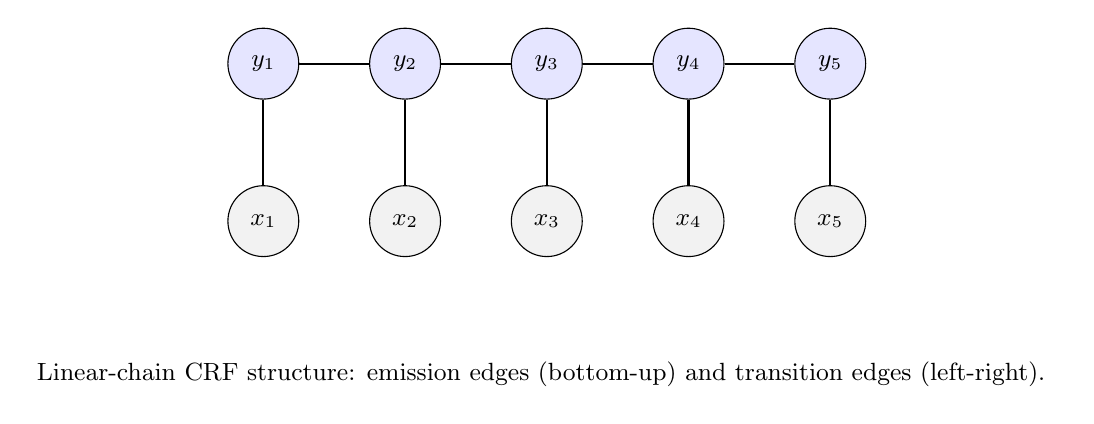
\begin{tikzpicture}[
    node distance=1.8cm,
    every node/.style={font=\small},
    obs/.style={circle, draw, minimum size=0.9cm, fill=gray!10},
    label/.style={circle, draw, minimum size=0.9cm, fill=blue!10},
    arrow/.style={->, thick, >=Stealth}
]

    % Observed tokens (x1 to x5)
    \node[obs] (x1) at (0,0) {$x_1$};
    \node[obs] (x2) [right of=x1] {$x_2$};
    \node[obs] (x3) [right of=x2] {$x_3$};
    \node[obs] (x4) [right of=x3] {$x_4$};
    \node[obs] (x5) [right of=x4] {$x_5$};

    % Labels above (y1 to y5)
    \node[label] (y1) at (x1) [yshift=2cm] {$y_1$};
    \node[label] (y2) at (x2) [yshift=2cm] {$y_2$};
    \node[label] (y3) at (x3) [yshift=2cm] {$y_3$};
    \node[label] (y4) at (x4) [yshift=2cm] {$y_4$};
    \node[label] (y5) at (x5) [yshift=2cm] {$y_5$};

    % Emission arrows (from x to y)
    \foreach \i in {1,...,5} {
        \draw[-, thick] (x\i) -- (y\i);
    }

    % Transition arrows (between y's)
    \foreach \i/\j in {1/2, 2/3, 3/4, 4/5} {
        \draw[-, thick] (y\i) -- (y\j);
    }

    % Caption
    \node[align=center, below=1.2cm of x3, font=\small] {
        Linear-chain CRF structure: emission edges (bottom-up) and transition edges (left-right).
    };

\end{tikzpicture}


    \caption[Linear-Chain CRF for Sequence Labeling]{Graphical representation of a linear-chain CRF used for sequence labeling.}
    \label{fig:crf-chain}
\end{figure}

\subsubsection{CRFsuite}
At first deployment, Conditional Random Fields had been used using the CRFsuite library, a lightweight yet effective structpred task framework for sequence labeling and other structured tasks~\cite{pythoncrfsuite}. This was a non-contextual baseline model, and it used only rich, handcrafted features and subword-level embeddings rather than deep contextual encoders.

The model input was a mixture of
\begin{compactitem}
\item \textbf{Handcrafted features}, borrowed from the AnyStyle parser, that mimic token-level features such as affixes, capitalization, punctuation, semantic category, and position.
\item \textbf{Byte-Pair Embeddings (BPEmb)}, providing subword-level semantic information for each token for most languages.
\end{compactitem}
These features were combined into a sparse, flat feature vector for each token in a target reference string. CRFsuite does not require vector embeddings as dense tensors such as neural models, but it accepts features in the form of string-labeled attributes, and therefore it is a viable choice for traditional sequence tagging with less computational need.
CRFsuite learns label dependencies through the sequence as well as inter-field transitions like \texttt{Author}, \texttt{Title}, and \texttt{Year}. However, it does not learn any context semantics through the sequence except label dependencies; no internal representation exists of the sequence content except in local features. Despite this, the combination of handcrafted linguistic features with BPEmb provided a respectable baseline in terms of accuracy as well as generalization.
The deployment was achieved with the assistance of the Python-CRFsuite library, which is a Python binding to CRFsuite offering a clean and expressive API for describing features and training CRF models.

\subsubsection{Neural CRF in PyTorch}
The second CRF implementation, i.e., Conditional Random Fields (CRF), used in this case is a neural variant integrated in a deep learning pipeline with PyTorch~\cite{torchcrf}. Unlike the CRFsuite-based model, which is specified over sparse feature vectors only, this implementation uses CRF as the output layer of a neural network. This allows the model to learn and use dense contextual embeddings while retaining the structured output behavior of traditional CRFs.
In this setup, each token in the input sequence is represented by a concatenated embedding vector comprising:
\begin{compactitem}
\item \textbf{Pretrained subword embeddings} (e.g., BERT or BPEmb),
\item \textbf{Trainable embeddings} from handcrafted categorical features.
\end{compactitem}
The pretrained embeddings are input to a Bidirectional LSTM (BiLSTM) encoder, which captures context across the entire sequence in both the forward and backward directions. The output of the BiLSTM — a contextualized representation for each token — is concatenated with the hand features, and then processed by a linear layer that produces emission scores for each label.
On top of the final layer, there is a CRF module that decodes the most likely sequence of labels by modeling the transition between tags. The module is trained jointly with the rest of the network under a negative log-likelihood loss, allowing the model to simultaneously learn emission as well as transition parameters.
This design benefits from both learned representations and structured sequence modeling. While the BiLSTM produces contextualized input embeddings, the CRF layer ensures that label predictions are in line with common citation patterns — e.g., ensuring that a B-Author label is not directly followed by a B-Year without an intervening I-Author.

The neural CRF was implemented using the torchcrf package, a widely used CRF layer for PyTorch that offers both training and decoding using efficient forward–backward algorithms.

\subsection{BiLSTM + CRF}
The BiLSTM + CRF architecture is among the most widespread and effective models for sequence labeling tasks, particularly if both label dependencies and contextual information are relevant. In this work, the BiLSTM is used to generate contextual embeddings of each token from subword representations, and the CRF layer embeds the dependencies between the output labels so that coherent predictions can be generated.

\subsubsection{BiLSTM Encoding}
LSTM networks are recurrent neural networks (RNNs) used to process long-range dependencies using gating mechanisms regulating information flowing through time~\cite{lstm}. Bidirectional LSTM reads the sequence in both directions, accessing context from future and previous tokens for each word~\cite{bilstm}. It is particularly useful in parsing the reference string, where the label of a token can depend on both the context before and after it.
In this design, the input to the BiLSTM is subword embeddings obtained from Byte-Pair Encoding (BPEmb). They offer semantics at the subword level and generalize for citation styles and languages. The BiLSTM outputs a sequence of hidden states for every token, representing its context-aware embedding.

\subsubsection{Integration of Handcrafted Features}
In addition to the subword embeddings, manually crafted features inspired by AnyStyle~\cite{anystyle} are used. Such categorical features are processed into a trainable embedding layer and projected to the same space as the BiLSTM representations. The two representations are combined using element-wise addition to form a fused vector that includes both learned and manually crafted knowledge.

\subsubsection{CRF Output Layer}
The combined representations are fed into a linear classifier to produce emission scores for each label. These are fed as input to a CRF layer that models label transitions and produces the most probable sequence using the Viterbi algorithm. The CRF is trained on a negative log-likelihood loss, which encourages it to produce high scores for valid and correct label sequences.

This model allows the system to take advantage of both deep contextualized representations and sequence-level coherence, and it is best suited for annotating structured references with highly diverse formatting styles.

\begin{figure}[ht]
    \centering
    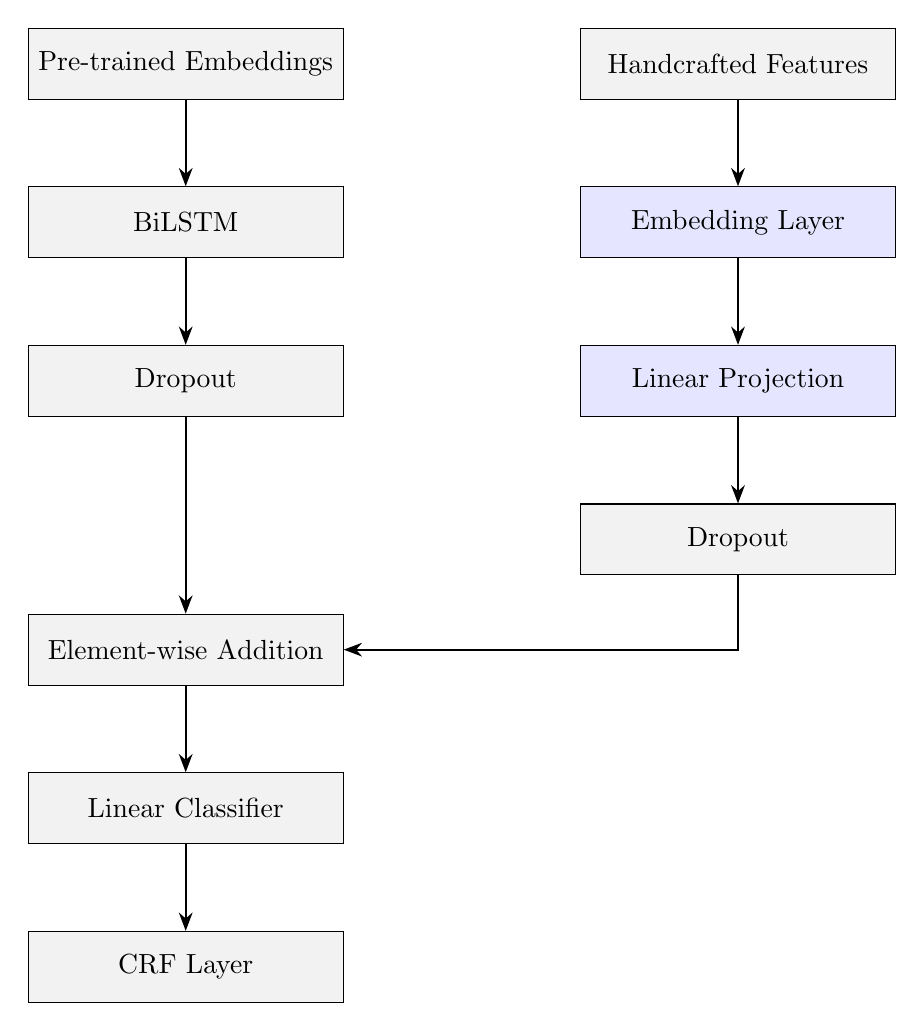
\begin{tikzpicture}[
    node distance=1.1cm,
    process/.style={rectangle, draw, minimum width=4cm, minimum height=0.9cm, align=center, fill=gray!10},
    embed/.style={rectangle, draw, minimum width=4cm, minimum height=0.9cm, align=center, fill=blue!10},
    arrow/.style={->, thick, >=Stealth}
]
    
    % Inputs
    \node[process] (bpe) {Pre-trained Embeddings};
    \node[process, below=of bpe] (lstm) {BiLSTM};
    \node[process, below=of lstm] (drop1) {Dropout};
    
    \node[process, right=3cm of bpe] (hand) {Handcrafted Features};
    \node[embed, below=of hand] (handemb) {Embedding Layer};
    \node[embed, below=of handemb] (proj) {Linear Projection};
    \node[process, below=of proj] (drop2) {Dropout};
    
    % Fusion
    \node[process, below=2.5cm of drop1] (add) {Element-wise Addition};
    
    % Output
    \node[process, below=of add] (linear) {Linear Classifier};
    \node[process, below=of linear] (crf) {CRF Layer};
    
    % Arrows: Left path (BPE → BiLSTM)
    \draw[arrow] (bpe) -- (lstm);
    \draw[arrow] (lstm) -- (drop1);
    \draw[arrow] (drop1.south) -- (add.north);
    
    % Arrows: Right path (Hand Features)
    \draw[arrow] (hand) -- (handemb);
    \draw[arrow] (handemb) -- (proj);
    \draw[arrow] (proj) -- (drop2);
    \draw[arrow] (drop2) |- (add.east);
    
    % Output path
    \draw[arrow] (add) -- (linear);
    \draw[arrow] (linear) -- (crf);
    
\end{tikzpicture}
    
    \caption[BiLSTM + CRF Model Architecture]{Architecture of the BiLSTM + CRF model combining pre-trained embeddings and handcrafted features.}
    \label{fig:bilstm-crf-architecture}
\end{figure}
\cleardoublepage

\section{Dataset and Preprocessing}
The accuracy of any machine learning algorithm, especially in sequence labeling problems, heavily relies on the quality and consistency of the input data. In this work, we use a vast corpus of citations to train and evaluate models to split and label reference strings into structured fields. This section describes the dataset used, the annotation and label formatting process, and the preprocessing pipeline that was developed to convert raw reference data into model inputs. Special attention is given to converting XML annotations into a standardized BIO tagging scheme and integrating both handcrafted and learned features.

\subsection{Dataset Description}
We employed the GIANT dataset~\cite{giant} to train as well as evaluate models for citation parsing in this research because it represents the largest public dataset of reference strings with annotations. The GIANT dataset came into existence to solve the problems of existing datasets due to their restricted nature of small sample size and limited domain applicability, while demonstrating minimal citation style variety. GIANT contains more than 991 million XML-labeled citation strings, allowing it to support modern deep learning approaches for reference string segmentation.

The research team developed GIANT through the amalgamation of three components:
\begin{compactitem}
\item 677,000 bibliographic records from Crossref,
\item The CSL repository contains 1,564 distinct citation styles, which form the basis of GIANT's data generation.
\item A widespread citation processor named citeproc-js served as the tool for formatting citations.
\end{compactitem}

Through citeproc-js, the entire Crossref database received transformation into every supported citation style. The produced citation strings underwent XML-style labeling that marked fields including \texttt{<author>}, \texttt{<title>}, \texttt{<year>}, and \texttt{<journal>} together with other tags. The team changed citation styles by hand to add the necessary tags that surrounded important bibliographic content for sequence labeling model use. By converting the documents into machine-readable format, the dataset contains a versatile collection of citation styles that range from journal articles to books and chapters, in addition to conference papers.
In total, the dataset includes:
\begin{compactitem}
\item \textbf{991,411,100 labeled citation strings}
\item Derived from \textbf{633,895 unique citations}
\item Spanning citation types such as:
\begin{compactitem}
\item Journal articles (75.9\%)
\item Book chapters (12.4\%)
\item Conference papers (5.6\%)
\item Others (e.g., datasets, reference entries)
\end{compactitem}
\end{compactitem}

All citations are in English, in the U.S. locale, and compressed for efficient retrieval. Every record also includes metadata such as citation type, citation style, and DOI. The metadata facilitates indexing and filtering, and researchers can focus on particular subdomains or types of citations when experimenting.

The scale and diversity of GIANT make it especially suited for training sequence labeling models such as CRFs and neural networks, which benefit from having both large numbers and varied examples. In this work, we used a 5 million sample subsample of GIANT due to computational constraints, selecting records uniformly across citation styles and types in order to preserve diversity.

\subsection{Label Set and Annotation Scheme}
The process of training citation parsing models needs each reference string to receive bibliographic field-specific labels. For our work, we have selected the BIO tagging format because it functions as a standard annotation method in sequence labeling tasks. The BIO scheme helps identify token positions within fields by using three labels, which represent  \textbf{Begin}, \textbf{Inside}, and  \textbf{Outside}. The starting words of \texttt{'Title'} receive label \texttt{B-Title}, yet succeeding words within the title use the label \texttt{I-Title}. Tokens without specification fall under the category \texttt{O}.
This data format proves being helpful in such applications because:
\begin{compactitem}
\item By using BIO it becomes simple to distinguish fields that extend across multiple consecutive tokens in cases such as lengthy author names and journal titles.
\item By using this format, models automatically acquire better capabilities for moving between different field categories.
\item CRF-based and neural sequence models with BIO-style labeling help the model to find complete compatibility when using this format.
\end{compactitem}

References in the original GIANT dataset receive full XML annotation for every listed field. A sample snippet includes different elements like \texttt{<author>}, \texttt{<given>}, \texttt{<family>}, \texttt{<title>}, \texttt{<issued>}, \texttt{<volume>}, \texttt{<container-title>}, \texttt{<page>} and \texttt{<URL>}, for example:
\begin{verbatim}
<author>
  <family>Ritchie</family>, <given>E.</given> and
  <family>Powell</family>, <given>Elmer Ellsworth</given>
</author>
(<issued><year>1907</year></issued>)
<title>Spinoza and Religion.</title>
<container-title>The Philosophical Review</container-title>,
<volume>16</volume>(<issue>3</issue>), p.
<page>339</page>. [online] Available from:
<URL>http://dx.doi.org/10.2307/2177340</URL>
\end{verbatim}

The detailed annotation scheme becomes complex for training models since multiple fields (such as \texttt{<given>} and \texttt{<family>}) need to merge into the \texttt{Author} category.
For this work, the annotated reference was simplified in an automated manner to retain only the most essential labels. These simplified labels were chosen to reflect the minimum necessary structure required to uniquely identify a cited work, while also keeping the annotation task manageable for a learning algorithm.
\begin{table}[h]
\centering
\begin{tabular}{ll}
\textbf{Label} & \textbf{Description} \\
\hline
Author & Names of authors, editors, or contributors \\
Title & Title of the work (book, article, etc.) \\
Container-Title & Journal, conference, or book series \\
Year & Year of publication \\
Volume & Volume number \\
Issue & Issue number (if available) \\
Page & Page number or page range \\
Publisher & Publishing organization or institution \\
DOI & Digital Object Identifier \\
ISSN & International Standard Serial Number (if available) \\
ISBN & International Standard Book Number \\
URL & Web link to the cited item \\
\end{tabular}
\caption{Simplified label set used for BIO tagging.}
\label{tab:labels}
\end{table}

\subsection{Preprocessing Steps}
Before training, a chain of preprocessing operations had been done on the raw GIANT dataset in order to prepare reference strings for sequence labeling. The data originally came in the form of XML-annotated data with mixed nested tags and unnecessary metadata. The pipeline below was applied in order to preprocess the training data into something clean and homogeneous:
\subsubsection{1. Tag Filtering and Simplification}
The original XML annotations contained a wide range of nested tags like \texttt{<given>}, \texttt{<family>}, and other irrelevant elements. A regular expression pattern was applied to extract all XML tags along with their values. A filtering step retained only a selected subset of allowed labels (e.g., \texttt{Author}, \texttt{Title}, \texttt{DOI}), and all the other tags were automatically removed.
This step of reducing tags made sure that only meaningful fields remained, but the job of annotation was still feasible for models. To remove nested tags, a recursive function was called, which left the valuable content and removed everything else.
\subsubsection{2. Cleaning Text}
Following tag filtering, the content left was flattened to plain text with labels implicit through XML tags for the permitted classes. Tokens were then processed for BIO annotation by regular expressions that:
\begin{compactitem}
\item Detect punctuation
\item Strip whitespace
\item Collapse nested or badly formed tags
\end{compactitem}
Each cleaned string was stored as an additional column alongside the original one, so that raw and processed inputs could be compared. 
\subsubsection{3. BIO Tagging}
Although not illustrated here in this phase, the reference strings that were cleaned were then tokenized and tagged in BIO format. The tokens were matched against the collapsed XML tags and tagged as \texttt{B-<TAG>} or \texttt{I-<TAG>}, based on their position within the field. Tokens that were not labeled were tagged with \texttt{O}.
\subsubsection{4. Splitting the Dataset}
Initial data files were read in from a subset of the GIANT dataset, shuffled using a set seed for reproducibility. Data was divided into:
\begin{compactitem}
\item 5 million training
\item 200k validation
\item 200k test
\end{compactitem}
This splitting was done similarly for all the samples to preserve type and style diversity.


\cleardoublepage

\section{Training and Evaluation Setup}
Two different training pipelines were used for the CRFsuite-based model and the BiLSTM+CRF model implemented in PyTorch. Both models were trained on processed data derived from the GIANT dataset, using subsets of varying size based on model complexity and resource constraints.
\subsection{CRFsuite Model}
The CRFsuite model was implemented using the sklearn-crfsuite Python library. Feature vectors for each token were constructed from a combination of handcrafted features and Byte-Pair Embeddings (BPEmb). These features were extracted and formatted into the string-keyed dictionary structure expected by CRFsuite.
\begin{compactitem}
\item \textbf{Training size:} 1 million \/ 5 million annotated reference strings
\item \textbf{Test size:} 100,000 \/ 200,000 references
\item \textbf{Optimizer:} Limited-memory BFGS (lbfgs)
\item \textbf{Regularization:} c1 = 0.1, c2 = 0.1
\item \textbf{Max iterations:} 100
\item \textbf{Transitions:} Enabled \texttt{all\_possible\_transitions} for richer label modeling
\end{compactitem}
The model was trained using default BIO-annotated labels. Model performance was evaluated using token-level metrics (precision, recall, F1-score) computed by flattening the sequences. The trained CRF model was serialized and stored using pickle for reuse and reproducibility.

\subsection{BiLSTM + CRF Model (Neural CRF)}
The BiLSTM + CRF model was implemented in PyTorch. It uses dense embeddings and contextual modeling, and was trained on a larger subset of the GIANT dataset due to its capacity to model long-range dependencies.
\begin{compactitem}
\item \textbf{Training size:} 5 million annotated reference strings
\item \textbf{Validation size:} 200,000 references
\item \textbf{Test size:} 200,000 references
\item \textbf{Batch size:} 32
\item \textbf{Dropout:} 0.5
\item \textbf{Optimizer:} Adam (torch.optim.Adam)
\item \textbf{Loss function:} Negative Log-Likelihood (from CRF layer)
\item \textbf{Embedding:}
\begin{compactitem}
\item Subword embeddings from BPEmb
\item Trainable embeddings from handcrafted feature classes
\end{compactitem}
\item \textbf{Architecture:}
\begin{compactitem}
\item Bidirectional LSTM followed by dropout
\item Projected handcrafted features added to LSTM output
\item Linear layer to generate emission scores
\item CRF layer for structured decoding
\end{compactitem}
\end{compactitem}

Datasets were loaded and batched using PyTorch's \texttt{DataLoader}, with a custom collate function that aligns token lengths and encodes categorical feature indices. Label-to-index mappings were handled dynamically based on the full BIO label set used in preprocessing.
Evaluation was conducted on the test set using the token-level F1-score and classification reports generated by \texttt{sklearn\.metrics\.classification\_report}.

\cleardoublepage
\cleardoublepage

\chapter{Results}
\label{ch:results}

\section{Evaluation Metrics}
For model performance evaluation, we employ the standard measures of \textbf{precision}, \textbf{recall}, and \textbf{F1-score} from sequence labeling tasks. These are calculated at the token level such that each token prediction is compared against its respective ground truth label. A prediction is considered correct only if both the BIO tag and the corresponding field label (e.g., \texttt{B-TITLE}, \texttt{I-YEAR}) match the reference string annotated.

The metrics are computed with the \texttt{classification\_report} function of the \texttt{sklearn.metrics} module, which provides a per-class breakdown, together with macro- and weighted averages across all labels:
\begin{compactitem}
\item \textbf{Precision} is the proportion of predicted tokens for a label that were accurate.
\item \textbf{Recall} is the proportion of actual tokens correctly predicted.
\item \textbf{F1-score} is the mean of precision and recall, offering a balance of performance.
\end{compactitem}
Because of class frequency imbalance (for example, \texttt{O} tokens and \texttt{I-TITLE} are far more common than \texttt{B-ISSN} or \texttt{I-ISSUE}), we present \textbf{macro averages} (which are treating all labels equally) and \textbf{weighted averages} (which treats class frequency), because due to given class frequency imbalance we want to emphasize both overall model robustness and infrequent field type performance.
For example, in the CRF model, token-wise weighted F1-score was 0.91 with particularly high performance for often occurring fields \texttt{B-AUTHOR}, \texttt{I-TITLE}, and \texttt{B-PAGE}. More underrepresented labels \texttt{I-ISSUE} and \texttt{I-ISBN} achieved modestly lower recall as might be expected relative to their frequency within the corpus.


\section{Model Comparison}
\subsection{CRF Configurations}
During the first phase of experimentation, we experimented with a baseline CRF model with input features having solely \textbf{Byte-Pair Embeddings (BPEmb)}. It was trained on a dataset of 1 million labeled reference strings and served as the baseline to study the performance of semantic subword embeddings in isolation for citation parsing.

To examine if the mere encoded token-level cues would improve performance, we enriched the feature set by adding \textbf{hand-engineered features} derived from the AnyStyle parser~\cite{anystyle}. These included affixes, punctuation type, character case, semantic class, and position. The new model, again trained on 1 million samples, utilized a concatenation of BPEmb and these additional features.
The result was substantial improvement across all field tags with the exception of the most common ones. Precisely, F1-scores on structurally ambiguous or poorly documented fields (e.g., \texttt{B-ISSUE}, \texttt{B-DOI}, \texttt{I-CONTAINER-TITLE}) increased, which suggests that hand-engineered features helped the model detect syntactic boundaries and semantic roles harder to acquire from embeddings.

Encouraged by this progress, we ramped up CRF training to leverage \textbf{5 million} annotated examples and preserve both handcrafted features and BPEmb. Increased training size brought additional improvements, particularly in label consistency and low-frequency tag recall.
This line of models — from embeddings-only, to hybrid features, to large-scale training — illustrates how both feature sparsity and training size lead to better structured prediction performance on citation parsing tasks.

The following table showes the results of each of the models and its performance on the test set:
\begin{table}[h]
    \centering
    \begin{tabular}{|c|c|c|c|}
    \hline
    \textbf{Model} & \textbf{Training Size} & \textbf{Features Used} & \textbf{F1-score (Weighted Avg)} \\
    \hline
    CRF & 1 million & BPEmb only & 0.87 \\
    CRF & 1 million & BPEmb + Handcrafted & 0.90 \\
    CRF & 5 million & BPEmb + Handcrafted & 0.91 \\
    \hline
    \end{tabular}
    \caption[CRF Model Comparison (Features and Sizes)]{Comparison of CRF models with different features and dataset sizes using weighted F1-score.}
    \label{tab:crf_comparison}
\end{table}

As shown in Table~\ref{tab:crf_comparison}, we observe a consistent improvement in F1-score as we increase the feature richness and training data size. Adding handcrafted features to the BPEmb baseline improves the model's ability to capture structural cues in citation strings. Further increasing the training data to 5 million references yields additional gains, highlighting the importance of both quality and quantity in feature-based CRF models.


\subsection{BiLSTM + CRF}
Two variants of the model were trained using \textbf{5 million reference strings}: one using only BPEmb, and the other using BPEmb with additional handcrafted features. Both models were evaluated on the same test set using token-level precision, recall, and F1-score. The results are summarized in Table~\ref{tab:bilstm_comparison}.
\begin{table}[h]
    \centering
    \begin{tabular}{|c|c|c|}
        \hline
        \textbf{Metric} & \textbf{BPEmb only} & \textbf{BPEmb + Hand} \\
        \hline
        Precision (Weighted Avg) & 0.80 & 0.83 \\
        Recall (Weighted Avg)    & 0.93 & 0.93 \\
        F1-score (Weighted Avg)  & 0.86 & 0.87 \\
        \hline
    \end{tabular}
    \caption[BiLSTM+CRF Feature Set Comparison]{Comparison of BiLSTM + CRF models trained on 5 million samples using different feature sets, the results are measured on the test set.}
    \label{tab:bilstm_comparison}
\end{table}

As shown in Table~\ref{tab:bilstm_comparison}, incorporating handcrafted features alongside BPEmb yielded a modest but measurable improvement in overall token-level F1-score. While both models benefited from the expressive power of bidirectional LSTMs, the inclusion of explicit structural cues contributed to more accurate field segmentation.

\subsection{BERT-based CRF Model}
To explore the effect of more advanced embeddings, we trained a CRF model using token-level embeddings generated by a modern \texttt{BERT-style encoder\\decoder}. Specifically, two different transformer-based architectures were evaluated:
\begin{compactitem}
\item \textbf{Linq-Embed-Mistral:} A recent multilingual model ranked highly on the Hugging Face embedding leaderboard for retrieval and semantic similarity tasks.
\item \textbf{DistilBERT Multilingual Cased:} A distilled and efficient version of BERT, offering faster inference with a modest trade-off in performance.
\end{compactitem}

Both models were used without additional handcrafted features or LSTM layers. The goal of these experiments was to determine whether high-quality contextual embeddings alone could match or surpass hybrid models that explicitly combine contextual and structural information.

The CRF models were trained on 5 million annotated reference strings using the BIO tagging scheme and evaluated using token-level precision, recall, and F1-score.
The results, summarized below, show that both BERT-based CRF models achieve competitive performance, with Linq-Embed-Mistral slightly outperforming DistilBERT in weighted F1-score. In particular, the Linq-Embed-Mistral model demonstrated superior performance on complex multi-token fields such as I-TITLE and I-AUTHOR, while DistilBERT achieved robust overall generalization with lower computational overhead. These findings suggest that leveraging strong pre-trained multilingual BERT based embeddings can effectively substitute for manual feature engineering when trained at scale.

\begin{table}[h] 
    \centering 
    \begin{tabular}{|c|c|c|} 
        \hline 
        \textbf{Metric} & \textbf{Linq-Embed-Mistral} & \textbf{DistilBERT} \\ 
        \hline 
        Precision (Weighted Avg) & 0.92 & 0.91 \\
        Recall (Weighted Avg)    & 0.94 & 0.93 \\
        F1-score (Weighted Avg)  & 0.93 & 0.92 \\
        \hline 
    \end{tabular} 
    \caption[BERT-based CRF Token-level Performance]{Token-level weighted F1-score performance of the CRF models using different BERT-style embeddings, the results are measured on the test set.} 
    \label{tab:bert_crf_comparison} 
\end{table}


\subsection{Final Comparison of Best Model Variants}
\label{subsec:final_comparison}
After analyzing each architecture independently, we summarize the performance of the best-performing configuration from each category in Table~\ref{tab:final_model_comparison}. The results clearly demonstrate the benefit of rich contextual embeddings provided by transformer-based models. The BERT + CRF configuration achieved the highest overall F1-score, followed by the traditional CRF using both BPEmb and handcrafted features. Interestingly, the BiLSTM + CRF model underperformed despite its ability to model sequential context, likely due to the difficulty of learning both token context and structure from scratch. This comparison highlights that pre-trained embeddings can substantially reduce the reliance on handcrafted features and outperform more complex neural architectures when applied effectively.
\begin{table}[h]
    \centering
    \resizebox{\textwidth}{!}{
        \begin{tabular}{|c|c|c|c|}
        \hline
        \textbf{Metric} & \shortstack{\textbf{CRF} \\ \textbf{BPEmb + Handcrafted}} & \shortstack{\textbf{BiLSTM + CRF} \\ \textbf{BPEmb + Handcrafted}} & \shortstack{\textbf{BERT + CRF} \\ \textbf{Linq-Embed-Mistral only}} \\
        \hline
        Precision (Weighted Avg) & 0.91 & 0.83 & 0.92 \\
        Recall (Weighted Avg)    & 0.91 & 0.93 & 0.94 \\
        F1-score (Weighted Avg)  & 0.91 & 0.87 & 0.93 \\
        \hline
        \end{tabular}
    }
    \caption{Final comparison between the best-performing models from each architecture family.}
    \label{tab:final_model_comparison}
\end{table}

\begin{figure}[H]
    \centering
    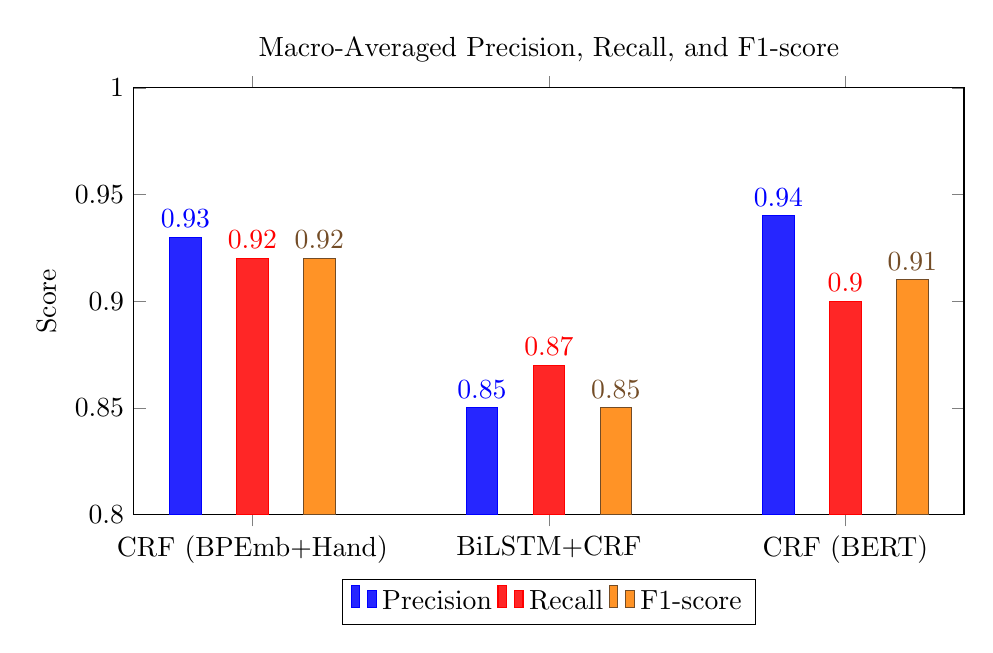
\begin{tikzpicture}  
    % Bar chart data
    \begin{axis}[
        ybar,
        bar width=.40cm,
        width=\textwidth,
        height=7cm,
        enlarge x limits=0.2,
        ylabel={Score},
        ymin=0.80, ymax=1.0,
        symbolic x coords={CRF (BPEmb+Hand), BiLSTM+CRF, CRF (BERT)},
        xtick=data,
        nodes near coords,
        nodes near coords align={vertical},
        legend style={at={(0.5,-0.15)}, anchor=north, legend columns=-1},
        xlabel={Model},
        title={Macro-Averaged Precision, Recall, and F1-score},
    ]
    \addplot+[style={fill=blue!85}, bar shift=-0.85cm] coordinates {
        (CRF (BPEmb+Hand),0.93) 
        (BiLSTM+CRF,0.85) 
        (CRF (BERT),0.94)
    };
    \addplot+[style={fill=red!85}, bar shift=0cm] coordinates {
        (CRF (BPEmb+Hand),0.92) 
        (BiLSTM+CRF,0.87) 
        (CRF (BERT),0.90)
    };
    \addplot+[style={fill=orange!85}, bar shift=0.85cm] coordinates {
        (CRF (BPEmb+Hand),0.92) 
        (BiLSTM+CRF,0.85) 
        (CRF (BERT),0.91)
    };

    \legend{Precision, Recall, F1-score}
    \end{axis}
\end{tikzpicture}
    \caption{Macro-level comparison of Precision, Recall, and F1-score across best-performing models.}
    \label{fig:model_comparison_chart}
\end{figure}

\subsection{Analysis of Results}
Based on the evaluation of the best-performing configurations across the CRF, BiLSTM + CRF, and BERT + CRF models, several insights can be drawn at both the macro and field-specific levels:
\begin{itemize}
\item \textbf{Model-Level Observations:}
\begin{compactitem}
\item \textbf{BERT + CRF}: achieved the highest overall weighted F1-score (0.93), along with the best precision (0.92) and recall (0.94). This confirms the effectiveness of transformer-based contextual embeddings, especially when used without additional handcrafted features.
\item \textbf{CRF (BPEmb + Handcrafted)}: performed surprisingly well with a weighted F1-score of 0.91, showcasing the strength of explicit token-level features when deep contextual embeddings are not available. Its performance was competitive with neural models across many fields.
\item \textbf{BiLSTM + CRF}, while offering contextual modeling through LSTM, slightly underperformed (F1-score: 0.87). This may be attributed to challenges in optimizing both the sequential context and structural features in a unified neural pipeline.
\end{compactitem}
\item \textbf{Field-Specific Insights:}
\begin{compactitem}
\item \textbf{Author Fields} (\texttt{B-AUTHOR}, \texttt{I-AUTHOR}): All models performed well on author detection, especially the BERT + CRF model, which reached F1-scores of 0.88 and 0.93 respectively. BiLSTM + CRF showed slightly lower precision on \texttt{B-AUTHOR}, indicating some sensitivity to name boundaries.
\item \textbf{Title Fields} (\texttt{B-TITLE}, \texttt{I-TITLE}): These fields consistently benefited from contextual embeddings. BERT + CRF achieved the best performance (\texttt{I-TITLE}: 0.94 F1), capturing long spans more effectively. The BiLSTM model also did well on \texttt{I-TITLE} due to its sequential memory, but struggled slightly with B-TITLE.
\item \textbf{URL Fields} (\texttt{B-URL}, \texttt{I-URL}): All models performed exceptionally on URLs, with F1-scores above 0.95. These fields are often easier to capture due to distinctive formatting (e.g., \texttt{http}, \texttt{www}, slashes), making them reliably detectable even by simpler models.
\item \textbf{DOI} and \textbf{PAGE}: Both BERT and CRF-based models achieved high performance on \texttt{B-DOI}, \texttt{B-PAGE}, and \texttt{I-PAGE}. These tokens also follow consistent patterns (numbers, slashes, etc.), allowing even non-contextual CRFs to generalize well.
\item \textbf{Container Title} (\texttt{I-CONTAINER-TITLE}): BiLSTM + CRF struggled here, achieving only 0.58 F1, while \textbf{CRF} and \textbf{BERT} models performed significantly better (0.87 and 0.85 respectively). This indicates that handcrafted features or pre-trained embeddings provide better signals for longer semantic chunks like journal names.
\item \textbf{Publisher} (\texttt{B-PUBLISHER}, \texttt{I-PUBLISHER}): The \texttt{I-PUBLISHER} tag was consistently well-handled across models (F1 near 0.90), but B-PUBLISHER showed more variability, reflecting challenges in distinguishing the beginning of organization names, especially when punctuation or unusual casing is involved.
\end{compactitem}
\end{itemize}

\subsection{Comparison with External Systems}
To place the performance of the new models in context, we compare their performance with previous work on bibliographic reference parsing. Despite potentially different conditions for datasets as well as evaluation policies, comparison provides an intuition of the relative position of the described methods.

\subsubsection{Evaluation Against a Large Language Model (GPT-4o)}
Recent advances in large language models (LLMs) have enabled strong performance on many natural language understanding tasks, even without explicit task-specific fine-tuning.
To explore how a general-purpose LLM would perform on bibliographic reference parsing, we used GPT-4o to label a sample of 100 reference strings.
The comparison offers insights into the strengths and limitations of applying a state-of-the-art LLM to a specialized sequence labeling task, without model retraining or task-specific adaptation.

Despite not having any task-specific tuning, GPT-4o did well on zero-shot general fields like \texttt{TITLE}, \texttt{PUBLISHER}, and \texttt{URL} with F1-scores greater than 0.90. Its performance was highly variable, however, on structured fields like \texttt{VOLUME}, \texttt{ISSUE}, \texttt{DOI}, and \texttt{ISBN}, where critical formatting details must be captured precisely. Our specialized models, however, like CRF with BPE and Handcrafted Features, BiLSTM+CRF, and CRF with BERT embeddings consistently outperformed GPT-4o across structured metadata fields. Overall, GPT-4o achieved a weighted F1-score of 0.89, while our best-performing models surpassed 0.91-0.93, confirming the value of task-specialized models for highly structured sequence labeling tasks like reference parsing.
\begin{figure}[H]
    \centering
    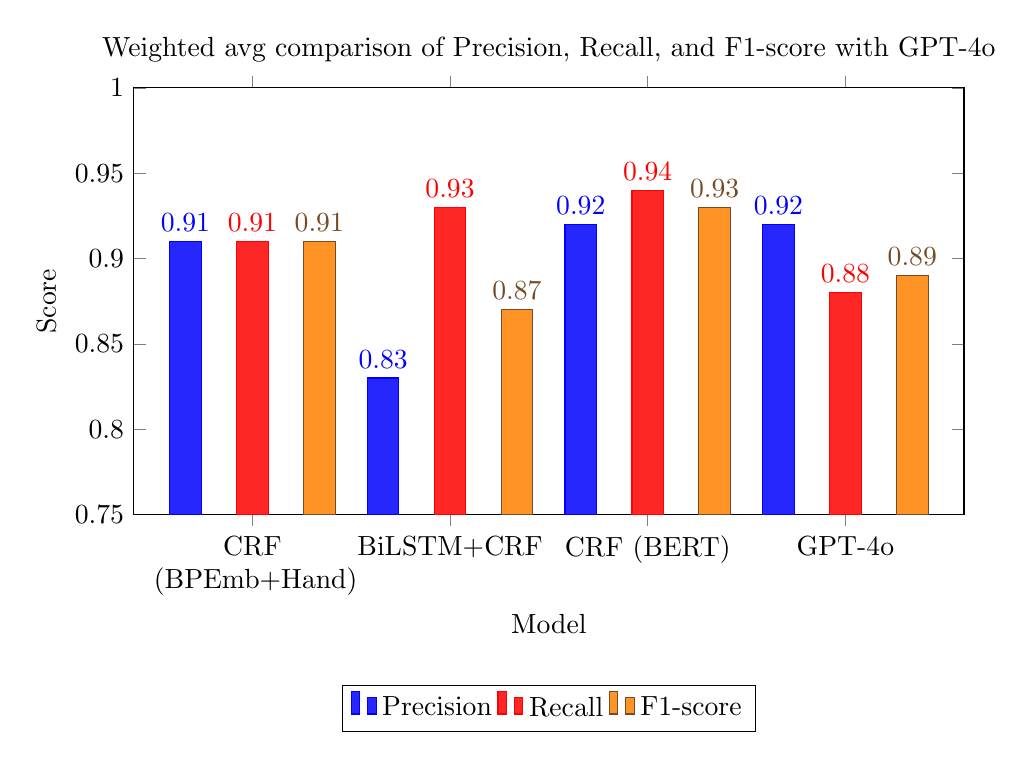
\begin{tikzpicture}
    \begin{axis}[
        ybar,
        bar width=0.40cm,
        width=\textwidth,
        height=7cm,
        enlarge x limits=0.2,
        ylabel={Score},
        ymin=0.75, ymax=1.0,
        symbolic x coords={CRF (BPEmb+Hand), BiLSTM+CRF, CRF (BERT), GPT-4o},
        xtick=data,
        xticklabel style={text width=2.5cm, align=center},
        nodes near coords,
        nodes near coords align={vertical},
        legend style={at={(0.5,-0.40)}, anchor=north, legend columns=-1},
        xlabel={Model},
        title={Weighted avg comparison of Precision, Recall, and F1-score with GPT-4o},
    ]
    
    \addplot+[style={fill=blue!85}, bar shift=-0.85cm] coordinates {
        (CRF (BPEmb+Hand),0.91) 
        (BiLSTM+CRF,0.83) 
        (CRF (BERT),0.92)
        (GPT-4o,0.92)
    };
    
    \addplot+[style={fill=red!85}, bar shift=0cm] coordinates {
        (CRF (BPEmb+Hand),0.91) 
        (BiLSTM+CRF,0.93) 
        (CRF (BERT),0.94)
        (GPT-4o,0.88)
    };
    
    \addplot+[style={fill=orange!85}, bar shift=0.85cm] coordinates {
        (CRF (BPEmb+Hand),0.91) 
        (BiLSTM+CRF,0.87) 
        (CRF (BERT),0.93)
        (GPT-4o,0.89)
    };
    
    \legend{Precision, Recall, F1-score}
    \end{axis}
\end{tikzpicture}
    \caption[Comparison of Best Models and GPT-4o]{Weighted-averaged Precision, Recall, and F1-score for the best performing models and GPT-4o.}
    \label{fig:comparison_gpt4o}
\end{figure}

\subsubsection{Comparison with External Published Work}
To put our models' performance into better perspective, we compare them to numbers published in independent studies. In particular, we compare our models' performance to the study by Cuéllar Hidalgo et al.~\cite{ArchComapre}, who have conducted an extensive evaluation of bibliographic reference parsing models. While their work shares some methodological similarity, the following key differences should be noted: their models were trained on much larger corpus (the full GIANT corpus), used no handcrafted features, and were evaluated on the CORA corpus — an independent test set from that employed in our experiments. Despite these differences, the comparison is worthwhile in so far as it gives insight into the relative design and performance of both approaches.

In their work, the BiLSTM+CRF model had a reported weighted F1-score of 0.96 while tested on the CORA dataset~\cite{ArchComapre} compared to both CRF-only and Transformer+CRF models. On our experiments, our top-performing BiLSTM+CRF model, which was trained using BPEmb embeddings and handcrafted features, achieved a weighted F1-score of 0.87 on our in-house large-scale test set. While our score is actually lower, note that our training set was much smaller (5 million references versus almost 200  million), and that hand-designed features were employed to augment performance instead of using learned embeddings exclusively.
Besides, while their evaluation used a standard dataset (CORA), our dataset more accurately sampled diverse and realistic styles of citations, with noisy and partial samples. This means our models retained good generalization behavior under more challenging situations.
\begin{figure}[H]
    \centering
    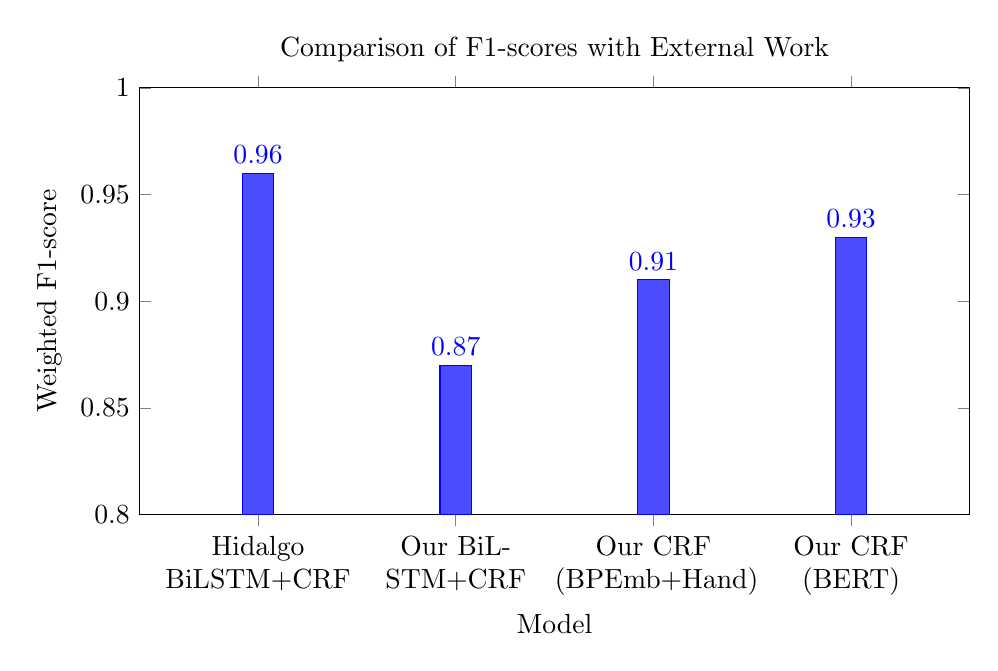
\begin{tikzpicture}
    \begin{axis}[
        ybar,
        bar width=.4cm,
        width=\textwidth,
        height=7cm,
        enlarge x limits=0.2,
        ylabel={Weighted F1-score},
        ymin=0.80, ymax=1.0,
        symbolic x coords={Hidalgo BiLSTM+CRF, Our BiLSTM+CRF, Our CRF (BPEmb+Hand), Our CRF (BERT)},
        xtick=data,
        xticklabel style={text width=2.5cm, align=center},
        nodes near coords,
        nodes near coords align={vertical},
        xlabel={Model},
        title={Comparison of F1-scores with External Work}
    ]
    \addplot+[style={fill=blue!70}] coordinates {
        (Hidalgo BiLSTM+CRF,0.96)
        (Our BiLSTM+CRF,0.87)
        (Our CRF (BPEmb+Hand),0.91)
        (Our CRF (BERT),0.93)
    };
    \end{axis}
\end{tikzpicture}
    \caption[Comparison of Weighted F1-Scores with External Published Work]{Comparison of weighted F1-scores between our models and the BiLSTM+CRF model from\cite{ArchComapre}.}
    \label{fig:external_comparison}
\end{figure}



\cleardoublepage

% \input{sections/user.tex}
% \cleardoublepage

% \input{sections/impl.tex}
% \cleardoublepage

% \input{sections/sum.tex}
% \cleardoublepage

% Acknowledgements (optional) - in case your thesis received funding or would like to express special thanks to someone
\chapter*{\acklabel}
\addcontentsline{toc}{chapter}{\acklabel}
I would like to express my heartfelt gratitude to my supervisor, \textbf{Simonyi András}, for his continuous support and insightful guidance throughout the course of this research. His expertise was instrumental in shaping the project and bringing it to completion.
I am also deeply thankful to the faculty and staff of the Department of Computer Science at Eötvös Loránd University, whose support and resources were essential to the successful execution of this work.
Finally, I extend my appreciation to the open-source community and the developers whose tools and libraries were integral to the implementation of this project.

% Appendices (optional) - useful for detailed information in long tables, many and/or large figures, etc.
% \appendix
% \input{sections/sim.tex}
% \cleardoublepage

% Bibliography (mandatory)
\phantomsection
\addcontentsline{toc}{chapter}{\biblabel}
\printbibliography[title=\biblabel]
\cleardoublepage

% List of figures (optional) - useful over 3-5 figures
\phantomsection
\addcontentsline{toc}{chapter}{\lstfigurelabel}
\listoffigures
\cleardoublepage

% List of tables (optional) - useful over 3-5 tables
\phantomsection
\addcontentsline{toc}{chapter}{\lsttablelabel}
\listoftables
\cleardoublepage

% List of algorithms (optional) - useful over 3-5 algorithms
% \phantomsection
% \addcontentsline{toc}{chapter}{\lstalgorithmlabel}
% \listofalgorithms
% \cleardoublepage
 
% List of codes (optional) - useful over 3-5 code samples
% \phantomsection
% \addcontentsline{toc}{chapter}{\lstcodelabel}
% \lstlistoflistings
% \cleardoublepage

% List of symbols (optional)
%\printnomenclature

\end{document}